\documentclass[twoside,openright,titlepage,numbers=noenddot,headinclude,footinclude=true,cleardoublepage=empty,BCOR=5mm,fontsize=10pt,dutch,english]{scrbook}
                     
\newlength{\mytextwidth}
\setlength{\mytextwidth}{288pt}

\newlength{\mytextheight}
\setlength{\mytextheight}{555pt}

\setlength{\footskip}{25pt}

\usepackage[papersize={17cm,24cm}, width=\mytextwidth, height=\mytextheight,hmarginratio={1:2},vmarginratio={1:1},bindingoffset=4mm]{geometry}

\PassOptionsToPackage{eulerchapternumbers,listings, pdfspacing, subfig,beramono,thesispaper}{classicthesis}					

\usepackage{ifthen}
\newboolean{enable-backrefs}
\setboolean{enable-backrefs}{false}

% Personal data
\newcommand{\myTitle}{Unsupervised Brain Anomaly Detection in MR Images\xspace}
\newcommand{\mySubtitle}{}
\newcommand{\myName}{Samuel Botter Martins\xspace}
\newcommand{\myUni}{University of Groningen\xspace}

% Setup and useful commands
\newcounter{dummy} 
\newlength{\abcd} 
\providecommand{\mLyX}{L\kern-.1667em\lower.25em\hbox{Y}\kern-.125emX\@}
\newcommand{\abbr}[1]{\textsc{\MakeLowercase{#1}}}

\newlength{\figureHalf}\setlength{\figureHalf}{139.74pt}
\newlength{\figureThird}\setlength{\figureThird}{90.32pt}
\newlength{\figureFourth}\setlength{\figureFourth}{65.61pt}

\newlength{\figureHalfBigSkip}\setlength{\figureHalfBigSkip}{129.8pt}
\newlength{\figureThirdBigSkip}\setlength{\figureThirdBigSkip}{77.0667pt}
\newlength{\figureFourthBigSkip}\setlength{\figureFourthBigSkip}{50.7pt}

% More packages
\usepackage{verbatim}
\usepackage{printlen}
\usepackage{makeidx}

\usepackage[lining]{libertine}
\usepackage[T1]{fontenc}
\usepackage{textcomp}
\usepackage[fleqn]{amsmath}
\usepackage{amsthm}
\usepackage[libertine]{newtxmath}
\usepackage{mathtools}
\usepackage[bb=pazo,bbscaled=0.94,cal=cm,calscaled=0.96]{mathalfa}
\usepackage{bm}
\usepackage{rotating}
\usepackage{mdframed}			% Create frames

% \usepackage[ruled,noline,noend]{algorithm2e}
% \usepackage[ruled,vlined,linesnumbered]{algorithm2e}
% \usepackage{algorithm}
\usepackage{algorithmic}

\renewcommand{\algorithmicrequire}{\textbf{Input:}}
\renewcommand{\algorithmicensure}{\textbf{Output:}}

\usepackage{sidecap}
\usepackage{marginnote}
\usepackage{tikz}
\usetikzlibrary{arrows,calc,positioning}
\usepackage{tabulary}

\usepackage{enumitem}

\newenvironment{myabstract}%
{\textsc{abstract:} \slshape\footnotesize }%
{}

\PassOptionsToPackage{utf8}{inputenc}	
 \usepackage{inputenc}				

\PassOptionsToPackage{dutch,english,portuguese}{babel}
 \usepackage{babel}					

\PassOptionsToPackage{square,numbers,sort&compress}{natbib}
% \PassOptionsToPackage{round}{natbib}
\usepackage{natbib}				

\usepackage{scrhack} % fix warnings when using KOMA with listings package          
\usepackage{xspace} % to get the spacing after macros right  
\usepackage{mparhack} % get marginpar right
\PassOptionsToPackage{printonlyused,smaller}{acronym}
	\usepackage{acronym} 
\ifdefined\bflabel
	\renewcommand{\bflabel}[1]{{#1}\hfill} % fix the list of acronyms
\else
\fi


% Setup floats: tables, (sub)figures, and captions
\usepackage{tabularx} % better tables
	\setlength{\extrarowheight}{3pt} % increase table row height
\newcommand{\tableheadline}[1]{\multicolumn{1}{c}{\spacedlowsmallcaps{#1}}}
\newcommand{\myfloatalign}{\centering} % to be used with each float for alignment
\usepackage{caption}
\captionsetup{format=hang,font=small}
\usepackage{subfig}  

%Setup code listings
\usepackage{listings} 
\lstset{language=[LaTeX]Tex,%C++,
    keywordstyle=\color{RoyalBlue},%\bfseries,
    basicstyle=\small\ttfamily,
    %identifierstyle=\color{NavyBlue},
    commentstyle=\color{Green}\ttfamily,
    stringstyle=\rmfamily,
    numbers=none,%left,%
    numberstyle=\scriptsize,%\tiny
    stepnumber=5,
    numbersep=8pt,
    showstringspaces=false,
    breaklines=true,
    frameround=ftff,
    frame=single,
    belowcaptionskip=.75\baselineskip
    %frame=L
} 

% PDFLaTeX, hyperreferences and citation backreferences
\PassOptionsToPackage{pdftex,hyperfootnotes=false,pdfpagelabels,breaklinks}{hyperref}
	\usepackage{hyperref}
\pdfcompresslevel=9
\pdfadjustspacing=1 
\PassOptionsToPackage{pdftex}{graphicx}
	\usepackage{graphicx} 
\usepackage[capitalise]{cleveref}

% Setup the style of the backrefs from the bibliography
\newcommand{\backrefnotcitedstring}{\relax}%(Not cited.)
\newcommand{\backrefcitedsinglestring}[1]{(Cited on page~#1.)}
\newcommand{\backrefcitedmultistring}[1]{(Cited on pages~#1.)}
\ifthenelse{\boolean{enable-backrefs}}%
{%
		\PassOptionsToPackage{hyperpageref}{backref}
		\usepackage{backref} % to be loaded after hyperref package 
		   \renewcommand{\backreftwosep}{ and~} % separate 2 pages
		   \renewcommand{\backreflastsep}{, and~} % separate last of longer list
		   \renewcommand*{\backref}[1]{}  % disable standard
		   \renewcommand*{\backrefalt}[4]{% detailed backref
		      \ifcase #1 %
		         \backrefnotcitedstring%
		      \or%
		         \backrefcitedsinglestring{#2}%
		      \else%
		         \backrefcitedmultistring{#2}%
		      \fi}%
}{\relax}    

% Hyperreferences
\hypersetup{%
    colorlinks=true, linktocpage=true, pdfstartpage=3, pdfstartview=FitV,%
    breaklinks=true, pdfpagemode=UseNone, pageanchor=true, pdfpagemode=UseOutlines,%
    plainpages=false, bookmarksnumbered, bookmarksopen=true, bookmarksopenlevel=1,%
    hypertexnames=true, pdfhighlight=/O,
    urlcolor=black, linkcolor=black, citecolor=black, 
    pdftitle={\myTitle},%
    pdfauthor={\textcopyright\ \myName},%
    pdfsubject={},%
    pdfkeywords={},%
    pdfcreator={pdfLaTeX},%
    pdfproducer={LaTeX with hyperref and classicthesis}%
}   

% Setup autoreferences
\makeatletter
\@ifpackageloaded{babel}%
    {%
       \addto\extrasenglish{%
					\renewcommand*{\figureautorefname}{Figure}%
					\renewcommand*{\tableautorefname}{Table}%
					\renewcommand*{\partautorefname}{Part}%
					\renewcommand*{\chapterautorefname}{Chapter}%
					\renewcommand*{\sectionautorefname}{Section}%
					\renewcommand*{\subsectionautorefname}{Section}%
					\renewcommand*{\subsubsectionautorefname}{Section}% 	
				}%
       \addto\extrasngerman{% 
					\renewcommand*{\paragraphautorefname}{Absatz}%
					\renewcommand*{\subparagraphautorefname}{Unterabsatz}%
					\renewcommand*{\footnoteautorefname}{Fu\"snote}%
					\renewcommand*{\FancyVerbLineautorefname}{Zeile}%
					\renewcommand*{\theoremautorefname}{Theorem}%
					\renewcommand*{\appendixautorefname}{Anhang}%
					\renewcommand*{\equationautorefname}{Gleichung}%        
					\renewcommand*{\itemautorefname}{Punkt}%
				}%	
			\providecommand{\subfigureautorefname}{\figureautorefname}%  			
    }{\relax}
\makeatother


\listfiles

\usepackage{classicthesis} 

% Further adjustments (experimental)
\usepackage{bibentry}
\nobibliography*

\providecommand{\doi}[1]{\abbr{DOI} \href{http://dx.doi.org/#1}{\urlstyle{same}\nolinkurl{#1}}}

\emergencystretch=1em

\newtheoremstyle{theoremStyle}
    {\topsep}                    % Space above
    {\topsep}                    % Space below
    {\itshape}                   % Body font
    {}                           % Indent amount
    {\scshape}                   % Theorem head font
    {.}                          % Punctuation after theorem head
    {.5em}                       % Space after theorem head
    {}  % Theorem head spec (can be left empty, meaning ‘normal’)
\theoremstyle{theoremStyle}
\newtheorem{theorem}{Theorem}
\newtheorem{lemma}[theorem]{Lemma}
\newtheorem{corollary}[theorem]{Corollary}
\newtheorem{proposition}[theorem]{Proposition}

\newtheoremstyle{exampleStyle}
    {0}                          % Space above
    {0}                          % Space below
    {}                           % Body font
    {}                           % Indent amount
    {\scshape}                   % Theorem head font
    {.}                          % Punctuation after theorem head
    {.5em}                       % Space after theorem head
    {}  % Theorem head spec (can be left empty, meaning ‘normal’)
\theoremstyle{exampleStyle}
\newtheorem{example}[theorem]{Example}
\usepackage{mdframed}
\surroundwithmdframed[bottomline=false,topline=false,rightline=false,
	linewidth=1pt,
	linecolor=gray,
	%innerleftmargin=7pt,
	skipabove=\topsep,
	skipbelow=0,
	innertopmargin=0,
	innerbottommargin=0]{example}

% Counters
\numberwithin{equation}{chapter}
\numberwithin{theorem}{chapter}
\numberwithin{figure}{chapter}

% CRef names
\crefname{algocf}{Alg.}{Algs.}
\Crefname{algocf}{Algorithm}{Algorithms}

\setlength{\marginparwidth}{8em}%

% Personal commands
\newcommand{\makenote}[1]{{ \color{red} [#1]}}

\DeclareMathOperator*{\argmax}{arg\,max}
\newcommand{\defaultwidth}{width=}

\DeclareMathOperator{\cov}{cov}
\DeclareMathOperator{\corr}{corr}
\DeclareMathOperator{\std}{std}
\DeclareMathOperator{\var}{var}
\DeclareMathOperator{\Val}{Val}

\DeclareMathOperator*{\KL}{KL}
\newcommand{\bs}{\bm}

\newcommand\independent{\protect\mathpalette{\protect\independenT}{\perp}}
\def\independenT#1#2{\mathrel{\rlap{$#1#2$}\mkern2mu{#1#2}}}

%% -----------------------------------------------
% My own commands
%% -----------------------------------------------

\newcommand{\fold}[1]{\mathcal{#1}}
\newcommand{\set}[1]{\mathbb{#1}}
\newcommand{\vecx}[1]{\boldsymbol{#1}}
\newcommand{\state}{\vecx{\phi}}

\newcommand{\chref}[1]{\autoref{ch:#1}}
\newcommand{\secref}[1]{\autoref{sec:#1}}
\newcommand{\figref}[1]{\autoref{fig:#1}}
\newcommand{\eqnref}[1]{\autoref{eqn:#1}}
\newcommand{\tabref}[1]{\autoref{tab:#1}}
\newcommand{\quadref}[1]{\autoref{quad:#1}}
\newcommand{\parref}[1]{\autoref{par:#1}}	
\newcommand{\coderef}[1]{\autoref{code:#1}}	
\newcommand{\appref}[1]{\autoref{app:#1}}
\newcommand{\itemref}[1]{\autoref{item:#1}}

\hypersetup{
	pdftitle={\myTitle}, 
	pdfauthor={\myName},
	pdfsubject={},
	pdfcreator={},
	pdfkeywords={}, 
	colorlinks=true,       		% false: boxed links; true: colored links
	linkcolor=blue,          	% color of internal links
	citecolor=blue,        		% color of links to bibliography
	filecolor=magenta,      	% color of file links
	urlcolor=blue,
	bookmarksdepth=4,
	plainpages = false,
  	linktocpage
}

% Just right frame
\newmdenv[leftline=false, topline=false, bottomline=false]{rightframe}

% Left and bottom frame
\newmdenv[topline=false, rightline=false]{leftbot}

% Top and bottom frame
\newmdenv[rightline=false, leftline=false]{topbot}

\newcommand{\hyp}[1]{
	\begin{topbot}
		\vspace{.5cm}	
		% \setlength{\parindent}{4em}
		% \setlength{\parskip}{2em}
		\noindent
		\emph{Hyphotesis: ``{#1}''}.
		\vspace{.5cm}
	\end{topbot}
}


%%%%%%% SAMUEL'S DEFINITIONS %%%%%%%%
\usepackage[ruled,vlined,linesnumbered]{algorithm2e}
\newcommand{\la}{\leftarrow}

\usepackage[]{appendix}
\usepackage{colortbl}
\usepackage{booktabs} 
\usepackage{hyperref}
\usepackage{multirow}
\usepackage{rotating}
\usepackage{subfig}
\usepackage{xprintlen}
% \printlen[2][cm]{\columnwidth} % to find out the column width in cm

% customizing colors from url, citations, and links
% RoyalBlue defined by the command \definecolor in classicthesis.sty
\hypersetup{%
	urlcolor=RoyalBlue,
	citecolor=RoyalBlue,
	linkcolor=RoyalBlue
}


% footnotes without numbers
\newcommand\blfootnote[1]{%
	\begingroup
	\renewcommand\thefootnote{}\footnote{#1}%
	\addtocounter{footnote}{-1}%
	\endgroup
}


\newcommand{\etal}{\emph{et al.}}
\newcommand{\eg}{\emph{e.g., }}
\newcommand{\ie}{\emph{i.e., }}

\newcommand{\fig}{Fig.}
\newcommand{\figs}{Figs.}

\newcommand{\tbf}[1]{\textbf{#1}}
\newcommand{\tit}[1]{\textit{#1}}
\newcommand{\mbf}[1]{\mathbf{#1}}

% review highlighting
\newcommand{\red}[1]{\textcolor{red}{#1}}
\newcommand{\blue}[1]{\textcolor{blue}{#1}}
\newcommand{\alex}[1]{\textcolor{red}{\textbf{Alex:} #1}}
\newcommand{\falcao}[1]{\textcolor{orange}{\textbf{Falcao:} #1}}
\newcommand{\samuel}[1]{\textcolor{magenta}{\textbf{Samuel:} #1}}


\newcommand{\adapro}{AdaPro\xspace}
\newcommand{\sosms}{SOSM-S\xspace}
\newcommand{\volbrain}{volBrain\xspace}
\newcommand{\malf}{MALF\xspace}

% \interfootnotelinepenalty=10000



%% Eduardo's additions
\usepackage[utf8]{inputenc}
\DeclareUnicodeCharacter{2010}{-}% support older LaTeX versions
\usepackage{rotating}
%% This fixes the section numbering that wasn't working but the font looks ugly
%% \RedeclareSectionCommands{section} 
%% Be careful here


\hyphenation{net-works}

\begin{document}

\sloppy

\frenchspacing
\raggedbottom
\selectlanguage{english}

\pagenumbering{roman}
\pagestyle{plain}

% Front matter
\begin{titlepage}
	\begin{addmargin}[-1cm]{-3cm}
    \begin{center}
        \large  

        \hfill

        \vfill

        \begingroup
            \color{Maroon}\spacedallcaps{\myTitle} \\ \bigskip
        \endgroup

        \spacedlowsmallcaps{\myName}

        \vfill

        \mySubtitle \\ \medskip   

        \vfill                      

    \end{center}  
  \end{addmargin}       
\end{titlepage}   
\thispagestyle{empty}

\hyphenation{}

\null
\vfill

\noindent Cover: add cover image description.
\vspace{1.5cm}

\noindent\myTitle\\
\hangindent=1em

\noindent \myName\\
PhD Thesis\\

\vspace{1.5cm}
\noindent This thesis is the result of a joint PhD between the Federal University of Rio Grande do Sul and the University of Groningen. \\

\vspace{1.5cm}

% TODO: ISBN when there is one
%\noindent \abbr{ISBN} 978-90-367-9288-2 (printed version)\\
%\abbr{ISBN} 978-90-367-9287-5 (electronic version)


\thispagestyle{empty}

\begin{addmargin}[-1cm]{-3cm}

\includegraphics[width=7.38cm]{figures/rugr_logoen_zwart_cmyk}

\begin{center}

\large 

\vfill\vfill\vfill\vfill\vfill

{\LARGE\textbf{\myTitle}}

\vfill\vfill\vfill\vfill\vfill

{\Large\textbf{PhD thesis}}

\vfill\vfill\vfill\vfill

to obtain the degree of PhD at the\\
University of Groningen\\
on the authority of the\\
Rector Magnificus Prof.\ C. Wijmenga\\
and in accordance with\\
the decision by the College of Deans,
and\\
to obtain the degree of PhD at the\\
University of Rio Grande do Sul\\
on the authority of\\
Rector Magnificus Prof.\ C. Bulhões Mendes.\\
\vfill
Double PhD Degree\\
\vfill

This thesis will be defended in public on\\

\vfill
% TODO: fill this when after room is reserved
Weekday DD Month YYYY at HH.MM hours\\

\vfill\vfill\vfill\vfill

by

\vfill\vfill\vfill\vfill

{\Large\textbf{\myName}}\\

\vfill
born on March 30th, 1995\\
in Porto Alegre, Brazil 
\end{center}
\end{addmargin}

\newpage
\thispagestyle{empty}
{\large
\noindent\textbf{Supervisors}\\
Prof. dr. Alexandru Cristian Telea\\
Prof. dr. João Luiz Dihl Comba\\

\noindent\textbf{Assessment committee}\\
Prof. Assessment prof1\\
Prof. Assessment prof2\\
Prof. Assessment prof3\\
Prof. Assessment prof4\\

\vfill
}


\pagestyle{scrheadings}

\cleardoublepage\null
\vfill

\hfill \begin{minipage}{.75\textwidth}
Just about anything looks better from a distance.

\hfill --- Haruki Murakami 
\end{minipage}

\cleardoublepage

\cleardoublepage\begingroup

\let\clearpage\relax
\let\cleardoublepage\relax
\let\cleardoublepage\relax

\manualmark
\markboth{\spacedlowsmallcaps{Abstract}}{\spacedlowsmallcaps{Abstract}} 
\phantomsection 

\pdfbookmark[0]{Abstract}{Abstract}
\chapter*{Abstract}

When it comes to tools and techniques designed to help understanding complex abstract data, visualization methods play a prominent role. They enable human operators to leverage their pattern finding, outlier detection, and questioning abilities to visually reason about a given dataset. Many methods exist that create suitable and useful visual representations of \emph{static} abstract, non-spatial, data. However, for \emph{temporal} abstract, non-spatial, datasets, in which the data changes and evolves through time, far fewer visualization techniques exist.

This thesis focuses on the particular cases of temporal hierarchical data representation via dynamic treemaps, and temporal high-dimensional data visualization via dynamic projections. We tackle the joint question of how to extend projections and treemaps to stably, accurately, and scalably handle temporal multivariate and hierarchical data. In both cases, the literature for the static techniques is rich and the state-of-the-art methods have proven to be valuable tools in data analysis. Their temporal/dynamic counterparts, however, are not as well studied, and, until recently, there were few hierarchical and high-dimensional methods that explicitly took into consideration the temporal aspect of the data. In addition, there are few or no metrics to assess the quality of these temporal mappings, and even fewer comprehensive benchmarks to compare these methods. 

This thesis addresses the abovementioned shortcomings. For both dynamic treemaps and dynamic projections. We propose ways to accurately measure temporal stability; we evaluate existing methods considering the tradeoff between stability and visual quality; and we propose new methods that strike a better balance between stability and visual quality than existing state-of-the-art techniques. We demonstrate our methods with a wide range of real-world data, including an application of our new dynamic projection methods to support the analysis and classification of hyperkinetic movement disorder data.

\newpage

\selectlanguage{dutch}

\manualmark
\markboth{\spacedlowsmallcaps{Samenvatting}}{\spacedlowsmallcaps{Samenvatting}} 
\phantomsection 

\pdfbookmark[0]{Samenvatting}{samenvatting}
\chapter*{Samenvatting}

Thesis abstract in Dutch.

\newpage

\selectlanguage{portuguese}

\manualmark
\markboth{\spacedlowsmallcaps{Resumo}}{\spacedlowsmallcaps{Resumo}} 
\phantomsection 

\pdfbookmark[0]{Resumo}{resumo}
\chapter*{Resumo}

Thesis abstract in Portuguese.

\selectlanguage{english}

\endgroup			

\cleardoublepage\begingroup
\let\clearpage\relax
\let\cleardoublepage\relax
\let\cleardoublepage\relax

\manualmark
\markboth{\spacedlowsmallcaps{Publications}}{\spacedlowsmallcaps{Publications}} 
\phantomsection 

\pdfbookmark[0]{Publications}{publications}
\chapter*{Publications}
This thesis is the result of the following publications:
\begin{itemize}
\item Quantitative Comparison of Treemap Techniques for Time-Dependent Hierarchies (poster) ~\citep{vernier17} \footnote{Best Poster Award at Eurovis 2017}
\item Quantitative Comparison of Dynamic Treemaps for Software Evolution Visualization~\citep{vernier18software} \footnote{Distinguished paper award at VISSOFT 2018}
\item A Stable Greedy Insertion Treemap Algorithm for Software Evolution Visualization~\citep{vernier18git}
\item Selecting and Sharing Multidimensional Projection Algorithms~\citep{EspadotoSharing}
\item Quantitative Comparison of Time-Dependent Treemaps~\citep{vernier_treemap}
\item Quantitative Evaluation of Time-Dependent Multidimensional Projection Techniques~\citep{Vernier2020}
\item Guided Stable Dynamic Projections~\citep{Vernier2021}
\end{itemize}


\endgroup

\cleardoublepage\refstepcounter{dummy}
\pdfbookmark[0]{\contentsname}{tableofcontents}

\setcounter{tocdepth}{4} 
\setcounter{secnumdepth}{4}

\manualmark
\markboth{\spacedlowsmallcaps{\contentsname}}{\spacedlowsmallcaps{\contentsname}}

\tableofcontents 

\automark[section]{chapter}
\renewcommand{\chaptermark}[1]{\markboth{\spacedlowsmallcaps{#1}}{\spacedlowsmallcaps{#1}}}
\renewcommand{\sectionmark}[1]{\markright{\thesection\enspace\spacedlowsmallcaps{#1}}}



% Main matter
\cleardoublepage
\pagenumbering{arabic}

\chapter{Introduction}
\label{ch:intro}
%
As science and technology evolves, a myriad of data collections are produced. The common denominator of all these data collections is the same -- they are regarded as containing useful and usable information from which actionable evidence can be extracted, the latter leading to improvements in many directions -- increased sales, better customer support, more accurate assessments of phenomena, or, at a higher level, the advance of understanding of these phenomena that have created the data, and, thereby, an increase of knowledge and advancement to science. These datasets challenge their consumers in many ways. Several relevant aspects that induce such challenges include the \emph{size} of datasets (the `big data' revolution has made the efficient processing of terrabyte dataset collections a mandatory requirement for most application areas); the \emph{quality} of data (principled statistical analysis and modeling of phenomena captured by data require accurately measured and collected datasets); and the \emph{provenance} of data (one needs to know how the entire end-to-end pipeline of obtaining a given dataset looks like before being able to make strong statements concerning insights derived from the respective data).

Yet, the challenges of understanding data are not limited to the above issues. A separate, and equally important, one regards the \emph{structure} of data itself. By structure, we mean here the relations that connect the measured data samples, also called observations or data points, so as to allow scientists to infer high-level considerations about the underlying phenomena. Data structure regards many aspects, including, but not limited to, the \emph{nature} of the data samples (\emph{e.g.}, these can be quantitative, categorical, text, relational, or multimedia types); the \emph{dimensionality} of the samples (how many independent attributes are measured to yield a single data sample); the \emph{temporality} of data (are the samples part of a single measurement of a phenomenon done at a single moment in time, or are they spread over a time range); and the \emph{organization} of the samples (do the samples create a flat, unstructured, set, or are they organized in a more refined manner, to denote a part-whole relationship).

Among many methods for data analysis, including statistics and machine learning, \emph{visualization} has a special place. Data visualization essentially leverages the skills of the human operator in \emph{e.g.} pattern finding, outlier detection, and at a higher level discovering unknown relationships between the data samples and thereby the ability to pose valuable questions by depicting the measured data via visual representations. Further on, data visualization can be enhanced by \emph{visual analytics}, which leverages the interactive dimension to allow human operators to view data from various angles, pose questions, and most importantly, formulate, check, and (in)validate hypotheses that ultimately lead to understanding the phenomena that have generated the data in the first place.

Data visualization -- and by extension, visual analytics -- can be roughly split into two main subfields. \emph{Scientific visualization} is traditionally concerned with the visual exploration of datasets consisting of samples having a relatively low number of dimensions (measurements). More importantly, these data points sample \emph{continuous} phenomena that cover the evolution of natural systems in the 2D or 3D space that describes our physical world, \emph{e.g.}, the flow of fluids, evolution of weather systems, the observable Universe, or chemical, anatomical, or medical phenomena embedded in their respective sciences. While far from having solved all problems in these fields, scientific visualization can exploit the 2D or 3D embedding of the measured samples, and, more importantly, exploit the continuous nature of the sampled phenomena, by using well-understood sampling, aggregation, statistical, and signal reconstruction methodology.

\emph{Information visualization} aims at leveraging the visual exploration power for all datasets which do not fall within the scientific visualization realm, meaning datasets where samples (a) do not reside in physical 2D or 3D space and/or (b) where the sampled dimensions are not necessarily continuous. An enormous realm of datasets, arguably larger than the scientific visualization ones, falls into this class. Examples include arbitrary data tables in any database or graphs and networks. Major challenges of information visualization stem precisely from the \emph{abstract} nature of the data it needs to depict: Since this data does not (usually) have a physical counterpart, it is (a) far less clear than for the scientific visualization case how to \emph{map} this data to suitable visual representations. On the other hand, by their very definitions, visualizations are perceived as continuous phenomena by users looking at them -- whether this regards the \emph{spatial} distribution of visual shapes drawn or the \emph{temporal} dynamics of how visualizations change over time as the depicted data changes. Since abstract data does not have an inherent continuity, the fundamental question arises on how to map non-continuous data to continuous visual representations for a good interpretation. Additional issues concerning big data, such as aggregation and sampling, only complicate the picture.

In this thesis, we attack a part of the above problem by focusing on abstract data that has three specific aspects:

\begin{itemize}
\item\emph{Hierarchical:} We consider data that can be organized into a hierarchy. Examples include files and folders stored on a hard disk, organigrams of people in an organization, or, more generally, any data that allows successive grouping and binning via multiple criteria;
\item\emph{High-dimensional:} We consider data whose samples consist of a large number (tens or more) of independently measured variablles, such as patient records, images treated by deep learning, or any data table having a large number of data columns;
\item\emph{Time-dependent:} We consider data that changes over time, also called \emph{temporal} or \emph{dynamic} data. Here, the samples of a dataset consist of both measurements taken at the same time instant and measurements taken at different, consecutive, time instants. 
\end{itemize}

In isolation, information visualization provides many methods to depict data which is hierarchical, high-dimensional, or temporal. However, the combination of at least two of the above three data aspects immediately makes the visualization problem far harder to address. In particular, we are interested on exploring how to visualize abstract datasets which are \emph{hierarchical and time-dependent}, respectively \emph{high-dimensional and time-dependent}. We outline the two separate challenges -- visualizing abstract data which is hierarchical and temporal, respectively high-dimensional and temporal, in Secs.~\ref{sec:ch1_tempo} and~\ref{sec:ch1_highdim} next.

\alex{You see I added quite a bit. Important: here and elsewhere: you NEED to go gently step-by-step and introduce/defend/explain the problem in SMALL increments.}

\eduardo{add necessary refs later}

\section{Visualizing temporal hierarchical data}
\label{sec:ch1_tempo}
%
Hierarchical datasets are trees, or hierarchies, with weighted nodes. Typically, weights are given for leaf nodes and computed for non-leaf nodes as the sum of their children's weights. One example of a hierarchical dataset is a computer's file system -- the ``shape of the tree'' is given by the organization of the directories, and the weight of the leaf nodes can be defined as a file attribute such as size. Many other examples exist. As already hinted at earlier in this chapter, virtually any tabular dataset can be reduced to such a hierarchy, by grouping rows (samples) successively on multiple criteria, each of them based on the similarity of the rows according to a given table column. Hence, any tabular dataset can lead to multiple hierarchies. Apart from that, inherently hierarchical datasets do exist, such as the file system example mentioned earlier.

The temporal aspect is introduced when data changes over time. Building upon the file system example, if we collect "snapshots", as in a Git repository or periodic backups of a hard drive, our data would be an evolving tree -- its organization (hierarchy) changes as we create and delete folders and files, and the weight of the leaf nodes change as files are edited.

There is a range of visual encodings suitable/designed for displaying hierarchical data, including node-link diagrams, icicle plots, sunburst plots, and, the focus of our research, \emph{treemaps}.
Given an input weighted tree, treemaps recursively partition a 2D spatial region into cells whose area (and possibly color, shading, and labels) encode the tree's data attributes. Treemaps have several major advantages compared to other visualizations of hierarchical data: They are visually compact -- every single screen pixel is used to convey data, which favors them for visualizing large hierarchies; and they are simple to understand.

Connecting back to our initial example, the first treemaping algorithm \citep{shneiderman92} was, in fact, designed for the purpose of displaying the contents and use of a file system by Ben Shneiderman:

\begin{quoting}
    "During 1990, in response to the common problem of a filled hard disk, I became obsessed with the idea of producing a compact visualization of directory tree structures. Since the 80 Megabyte hard disk in the HCIL was shared by 14 users it was difficult to determine how and where space was used. Finding large files that could be deleted, or even determining which users consumed the largest shares of disk space were difficult tasks".
\end{quoting}

Compared to other hierarchical visualization methods, treemaps scale well, making use of all available screen pixels to show data and thus able to handle trees of thousands of nodes. As Shneiderman realized when trying to reason and make decisions about the use of space in his lab's hard drives:
\textit{"Tree structured node-link diagrams grew too large to be useful, so I explored ways to show a tree in a space-constrained layout."}

Over the years, a range of different treemapping techniques was proposed, each designed to optimize different goals such as cell aspect ratio of cells (tied to readability), order preservation, similarity-based placement, and portrayal of uncertainty. The most common form of treemaps are rectangular treemaps, but a range of alternative models exist, such as Voronoi treemaps~\citep{balzer05,balzer05b}, orthoconvex~\citep{deberg14}, Bubble~\citep{bubble}, and Jigsaw treemaps~\citep{jigsaw}.

Yet, not much work has been done regarding dynamic treemaps, that is, treemap methods designed to portray temporal hierarchical datasets ensuring that temporal coherence is kept. In other words: While treemaps work well for depicting any (large) hierarchical dataset, when one adds the requirement that the data is changing, we do not know whether, and how, to use or adapt treemaps to display such data. As hinted at in the beginning of this chapter, a major issue here is the \emph{continuity} aspect: As data changes, so will treemaps that depict it. However, how to ensure that what a user sees in terms of visualization changes (in the treemaps) faithfully conveys the change in the underlying data? This is a major requirement for using treemaps for dynamic data. Indeed: If a dataset changed a lot, but the corresponding dynamic treemap visualization would not, then the user would get the false feeling that the data is not changing when it actually does. Conversely, if a dataset changed little over time, but the corresponding dynamic treemap visualization exhibited major changes between its different snapshots (corresponding to different measurement moments of the hierarchical data), the user would get the false feeling that data is changing a lot when it actually does not. In both above examples, we would have clear cases of \emph{false negatives}, respectively \emph{false positives} (related to interpreting change in the visualization), which are both detrimental for the added value of a visualization. While the above problems are known and recognized, there are no clear solutions to designing treemap algorithms to address them for dynamic data. This is our first key research question (detailed next in this chapter).

% \begin{figure*}[]
%     \centering
%     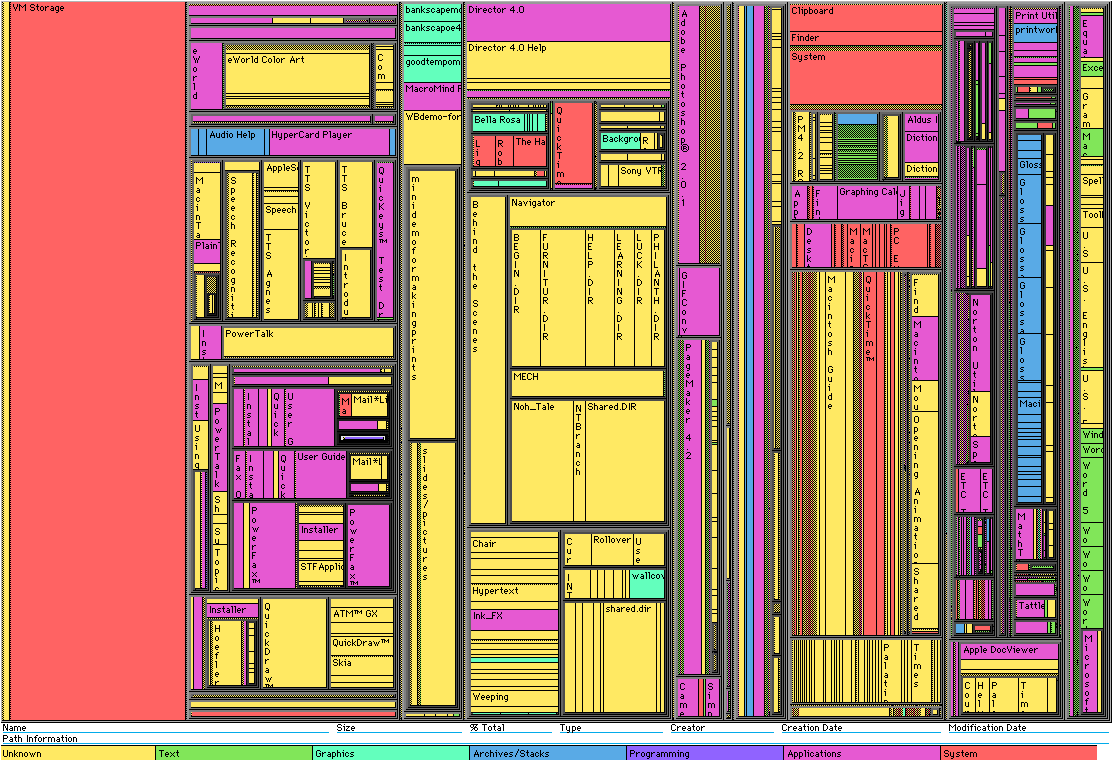
\includegraphics[width=.8\textwidth]{figures/intro/treemap_snd_colorful.png}
%     \caption{Earliest treemap method, Slice-and-Dice, displaying a file system.}
% \end{figure*}

\section{Visualizing temporal multidimensional data}
\label{sec:ch1_highdim}
%
Multidimensional (or high-dimensional) datasets have a number of observations (also called points or samples) where each observation has many attributes, also called variables, dimensions, or measurements. 
For datasets with relatively small numbers of observations and dimensions, techniques such as glyphs, parallel coordinate plots, table lenses, and scatterplot matrices can produce accurate and useful visual encodings.  
If a dataset has a large number of dimensions, roughly more than 4 to 5, however, multidimensional \emph{projections} tend to be the only scalable approach.  

Multidimensional projections take data in a high-dimensional space and project it into a lower-dimensional space, usually creating a 2D or 3D scatter plot, which we can directly visualize and reason about. In this transformation, the projection method attempts to create visual patterns that reflect the similarities or structure found in the high-dimensional space. That is, points which are similar -- according to any suitable similarity metric -- in the high-dimensional space are placed close in the 2D or 3D projection, and conversely.

Reflecting the similarities or structure found in the high-dimensional space can be interpreted in many ways, and the search for the ``best'' projection method has led to the proposal of a huge number of projection techniques.
There are many desirable traits projection methods can have, such as creating high distance or neighborhood preservation maps, scalability, simplicity, interpretability, out-of-sample capability, stability, and ease of use, among others. 
Optimizing a single one of these traits is already a challenging task that requires tradeoffs regarding the remaining traits. No single current method optimally satisfies all desirable requirements.

The trait that concerns us most in this thesis is \emph{stability}. Stability, or temporal coherence, needs to be taken into account when we project \emph{temporal} multidimensional data, that is, when the multidimensional data changes over time and, as illustrated in the previous section, we have multiple snapshots of the data. Most projection techniques are designed for static data. When used for time-dependent data, they usually fail to create a stable and suitable low dimensional representation. To follow the analogy with the dynamic treemaps discussed in Sec.~\ref{sec:ch1_tempo}: If we have a high-dimensional and temporal dataset, current projection methods usually create a visualization in which the observed points either do not change much while their corresponding high-dimensional counterparts change a lot; or they do change a lot whereas the high-dimensional data points only change little. Globally, the problem with projections is the same as that of treemaps -- they can produce false negatives and/or false positives which impair the ability of the user to judge about the data dynamics from seeing the visualization of the projected data.

\section{Temporal coherence}
\label{sec:ch1_coherence}
%
Treemaps and projections are incredibly useful techniques that, due to their compact and easy to interpret design, give unique insights into large and complicated datasets.
As mentioned so far, they were initially designed for static datasets. However, given the presence of dynamic datasets, the natural question arises on how to adapt them to handle such data, while avoiding the already discussed false-negative and false-positive problems. 

To illustrate the dynamic projections' instability, Fig.~\ref{fig:intro-pj-demo-instability} shows three different methods (G-PCA, TF-PCA~\citep{pca}, and TF-tSNE~\citep{tsne}) projecting the same dataset, using a trail-like visual encoding. The \emph{gaussians} dataset is a 100-dimensional dataset of 2000 samples covering 10 distinct isotropic Gaussian distributions that collapse into 10 single points over 10 timesteps. Knowing the dataset, we can tell that G-PCA renders quite faithfully the data dynamics and structure; TF-PCA creates an artificial amount of spiraling; and TF-tSNE creates a very large amount of apparently random and unstable motion that is not present in the data.  For the purpose of the illustration in Fig.~\ref{fig:intro-pj-demo-instability}, detailed knowledge of the G-PCA, TF-PCA, and TF-tSNE projection methods is not needed. The point being made is that different projection methods show widely different visual insights in the \emph{same} dataset. As such, they clearly cannot be all right -- raising the question of which method is the best and, subsequently, how to define what a good method is in this context.

% https://docs.google.com/drawings/d/1XENnHkpmsl6AqJfx5l2b-H4bSuKonbjgjYY_E599Q5c/edit
\begin{figure*}[h]
    \centering
    \includegraphics[width=\linewidth]{figures/projection-algorithm/demo-instability-trails-rebuttal-with-color-3.eps}
   %  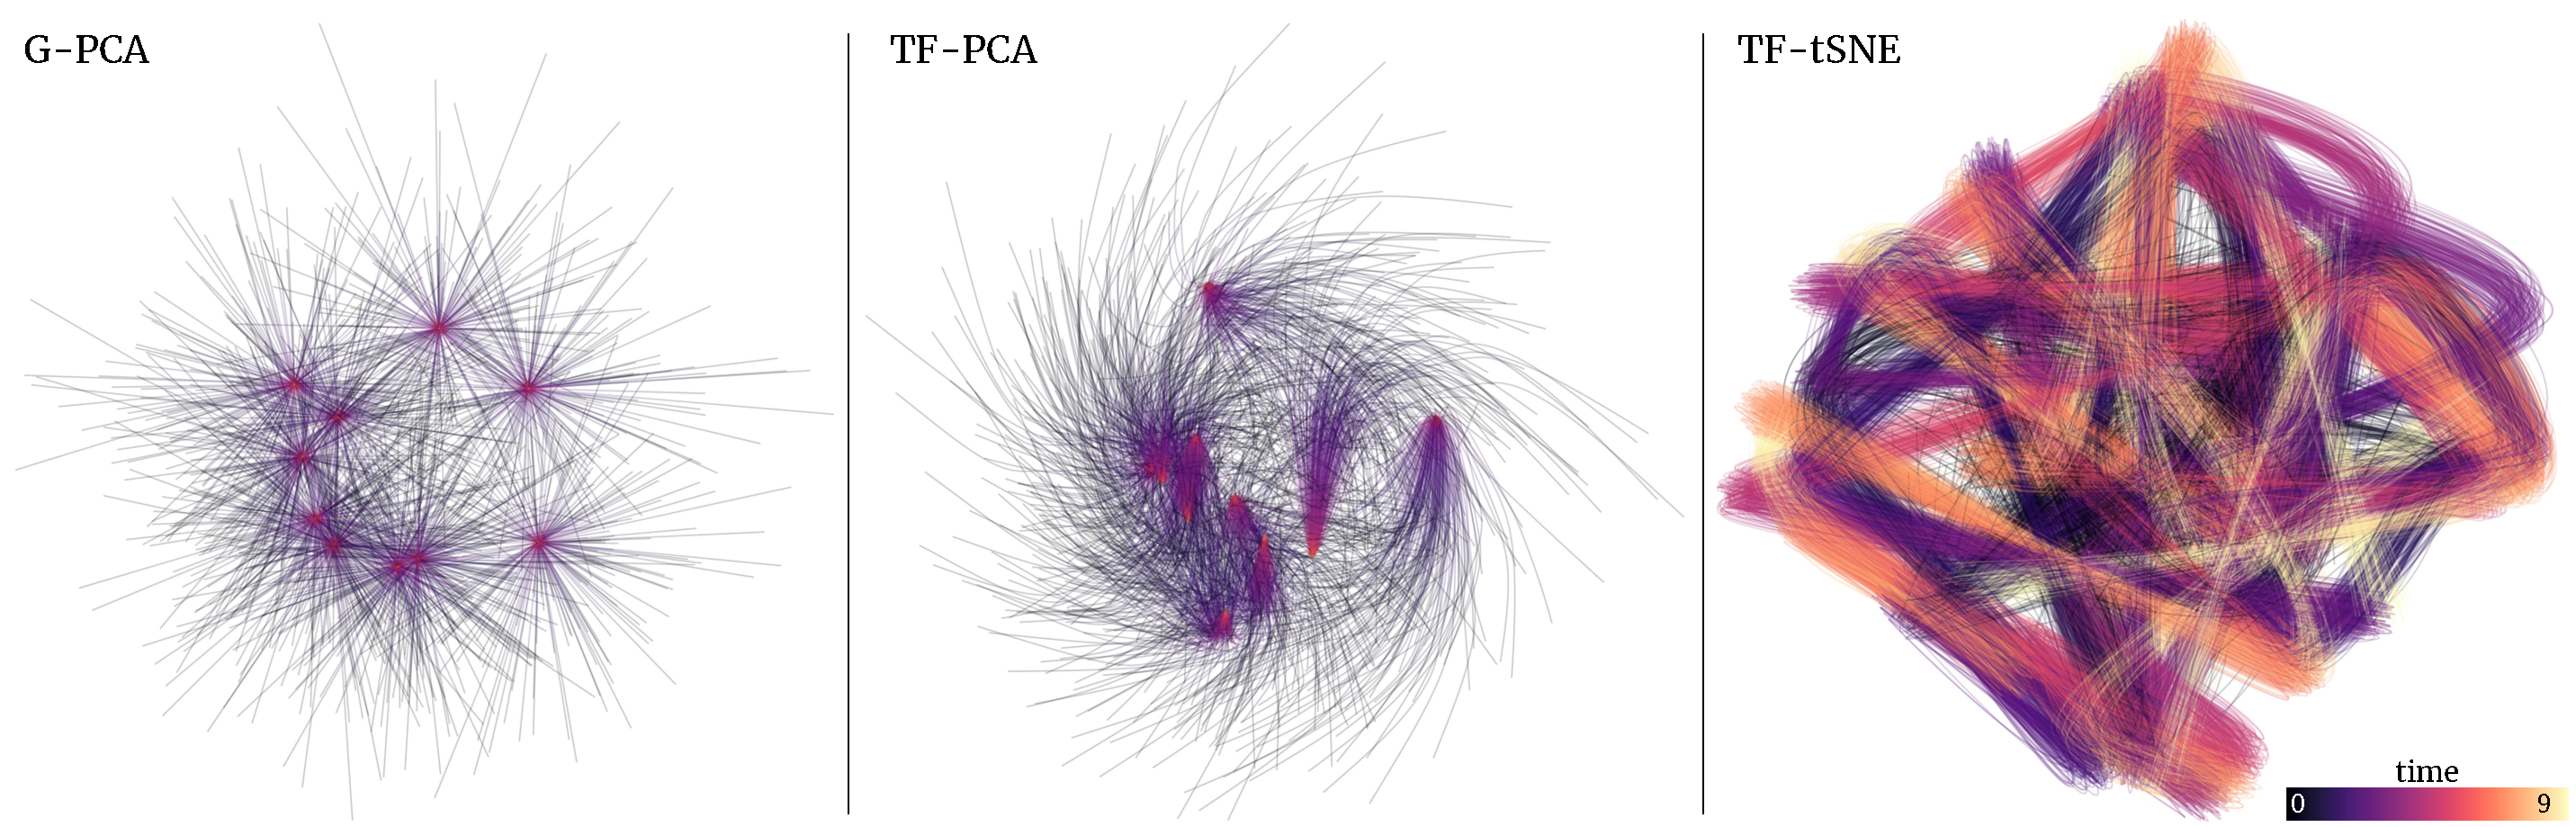
\includegraphics[width=0.48\linewidth]{figures/projection-algorithm/demo-instability-trails-rebuttal-with-color.pdf}
    \caption{A time-dependent collapsing 100-dimensional 10-Gaussian-distributions dataset (2000 points) from \cite{Rauber2016} is visualized by three projection methods. Point trails are colored by time (top) and class (bottom). The images show increasing amounts of instability artefacts.}
    \label{fig:intro-pj-demo-instability}
\end{figure*}

The same effect occurs when we create treemaps for time-dependent datasets. The top row of Fig.~\ref{fig:intro-tm-demo-instability} shows three snapshots/timesteps of the evolution of a simple weighted tree. The next two rows show two different treemapping algorithms creating rectangular treemap representations for the data (NMap and Squarified Treemap). Nmap creates a stable layout; that is, there are no significant changes in the positions of the cells driven by the small changes in the data, and the adjacencies in the layout remain the same over the evolution. In contrast, in the Squarified Treemap layout, cell \emph{d} (red) keeps changing its relative position. When dealing with more complicated datasets, this movement can happen for multiple cells simultaneously, making it impossible to accurately reason about the data and the change in the data. As for the projection example in Fig.~\ref{fig:intro-pj-demo-instability}, the issue is not understanding how NMap or Squarified Treemap work. Rather, the higher level question is that (at least) one of these methods is suboptimal, and, as a consequence, how to measure the quality of a dynamic treemapping method.

\begin{figure*}[h]
    \centering
    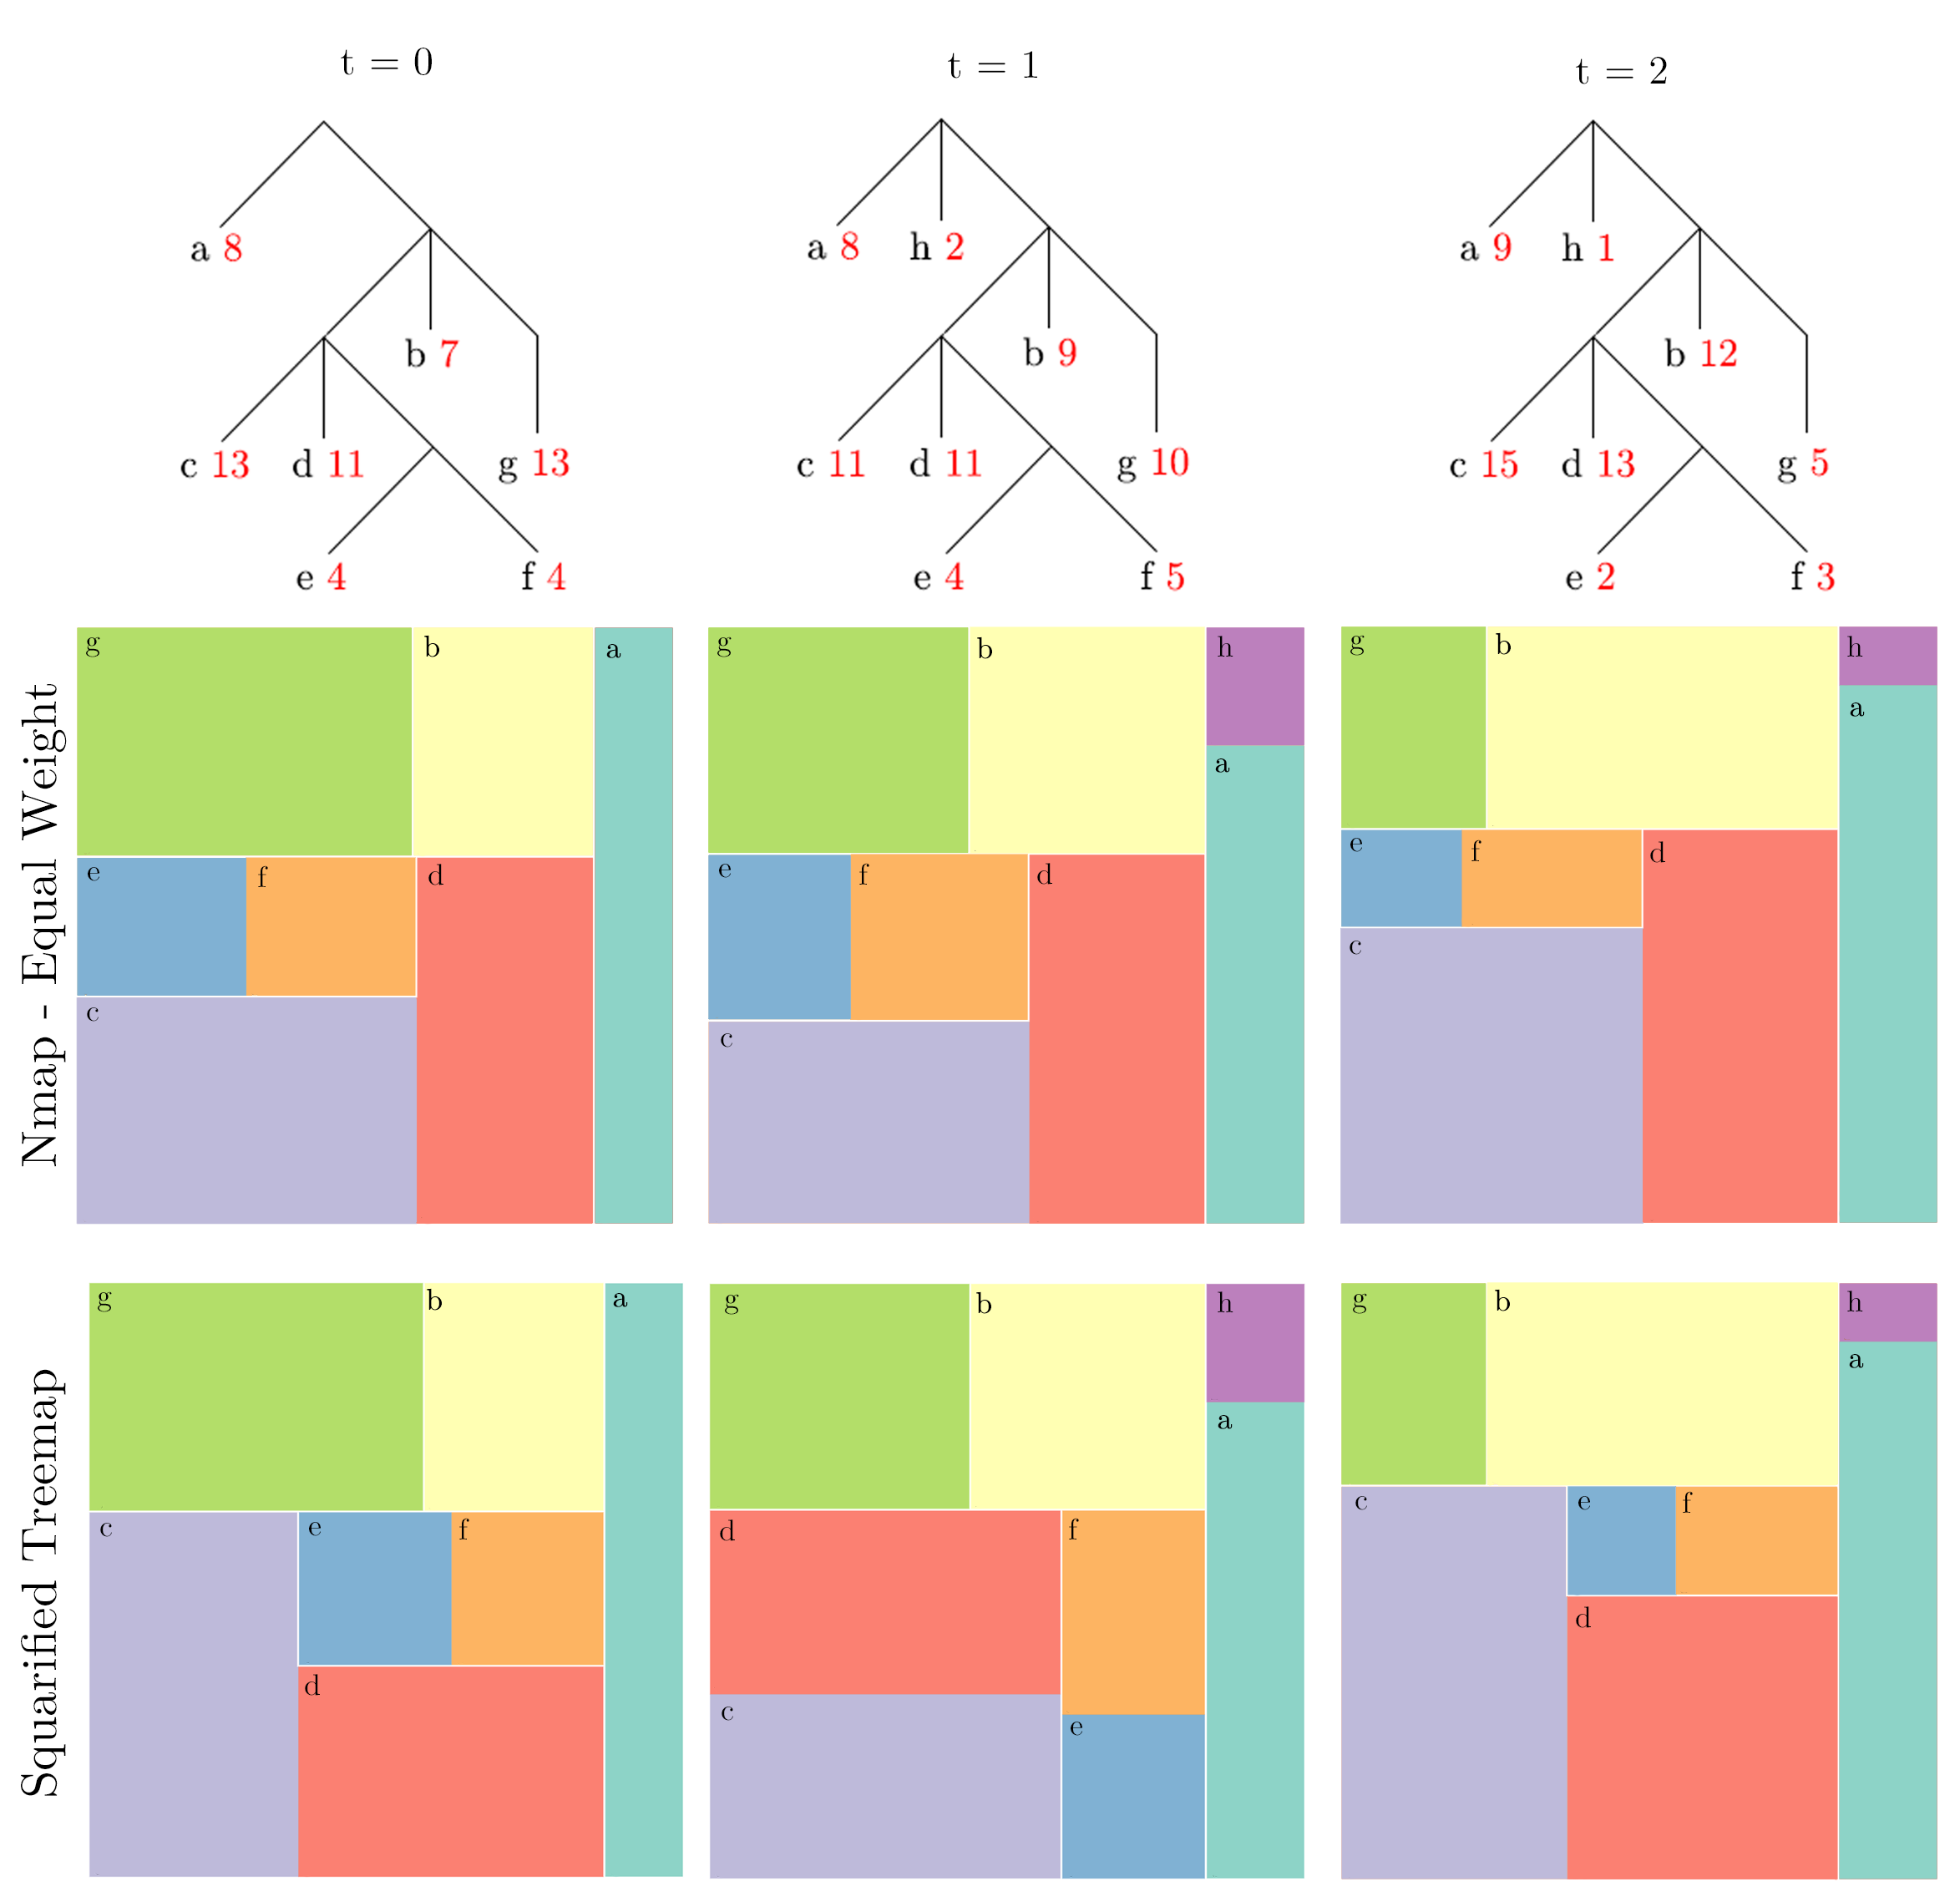
\includegraphics[width=\linewidth]{figures/intro/mov_sub_new.png}
    \caption{Layouts generated by NMap\,\citep{nmap} and Squarified Treemap\,\citep{sqr} for a sample hierarchical dataset
    of 3 time steps. We see how NMap is more stable, and similar in aspect ratio, than Squarified Treemap.}
    \label{fig:intro-tm-demo-instability}
\end{figure*}

To create faithful and useful representation of temporal data, we need to be able to ensure \emph{temporal coherence}: Small changes in the data should result in small changes in the visualization; large changes in the data should result in large changes in the visualization. All other mappings of changes in the data to changes in the visualization are arguably bad. Simply put, we want to guarantee that changes perceived by the viewer are due to changes in the data alone. However, while this 
desiderate is -- we argue -- clear and evident, there are no treemapping or projection algorithms that comply with it. Even more fundamentally, the very issue of relating data change to visualization change in these two contexts, and deciding what is a `good' mapping of the former to the latter, is not defined by theory or metrics to gauge it.

\section{Objectives and contributions}

We have argued that treemaps and projections are valuable tools for making sense of hierarchical and multidimensional data, respectively. However, when it comes to applying these visual encodings to \emph{time-dependent} data, these methods tend to show undesirable traits; and only limited research effort has been dedicated to understanding, testing, and developing methods that preserve temporal coherence. This research gap leads us to this thesis' high-level research question, stated next as

\subsection*{How to extend projections and treemaps to stably, accurately, and scalably handle temporal multivariate and hierarchical data?}

To address this question, there are three components that must be satisfied in either track. We must be able to

\subsection*{A. Develop ways of accurately measuring stability}

To evaluate the stability of a dynamic treemap or dynamic projection, we need to have reliable measurement tools that quantify the relationship between data change and visual change.

For treemaps, we developed the \emph{Unavoidable Change} \citep{vernier18software} metric, based on the mathematically proven minimum change that cells would need to undergo to accommodate the data change, and \emph{Baseline Treemaps} \citep{vernier_treemap}, a similar method to approximate the minimum amount of change that any time-dependent treemap must incur when data changes. We also proposed a set of stability metrics for dynamic projections based on the mathematics of visual quality metrics.
Before our work, there were no methods designed to measure instability that took into consideration data change -- they only looked at visual change, which can be deceiving. As such, we argue that our work provides a contribution to the fundamentals of using treemaps for reliably depicting dynamic hierarchical data.

\subsection*{B. Evaluate methods in the literature considering the tradeoff between stability and visual quality}

As already hinted, tens of methods for constructing treemaps and projections exist. However, and as also already hinted, few if none of these methods were gauged from the perspective of stability -- one reason thereof being the lack of a \emph{measure} for stability. Having developed such a measure, as mentioned above at point (A), we next use it to produce comprehensive evaluations for dynamic treemaps and projections from the stability perspective. Our contributions in this direction entail work along the following axes:

\begin{itemize}
    \item \emph{Metrics:} We proposed and implemented a novel set of metrics that reliably measures visual quality and stability.
    \item \emph{Datasets:} Since there was no previous extensive evaluation or benchmark designed for testing dynamic treemaps or projections, we collected and/or generated a comprehensive collection of datasets that drove our evaluations. 
    \item \emph{Methods:} Collection, implementation, and proposal of several dynamic treemap and projection algorithms. Most of the work on the topic up until our work was conjectural and not quantitatively tested.  Simply put, there was no central collection of algorithms that one could use to compare and gauge the performance of dynamic treemaps and dynamic projections. We claim that work solved a large part of this challenge.
    \item \emph{Analysis:} We combined the previous axes into comprehensive insights into dynamic projections and treemaps. Simply put, we generated quantitative and qualitative evidence showing how existing dynamic projection and treemap algorithms compare to each other, allowing both researchers and practitioners to choose which subset of algorithms are best suited to extend next, respectively directly use in practice.
\end{itemize}

\subsection*{C. Design state-of-the-art methods that strike a good balance between stability and visual quality}

Once the tools necessary to test and compare dynamic treemaps and projections were in place, we were able to leverage the gained insights to produce state-of-the-art algorithms that strike a better balance between stability and visual quality.

Specifically, we have developed Greedy Insertion Treemap (GIT) \citep{vernier18git}, a stable and scalable state-aware method for displaying dynamic treemaps. Compared to all treemapping algorithms that we were aware of at the time of GIT's development, we showed that GIT provides a better tradeoff between spatial quality and stability, therefore surpassing its competitors. Moreover, GIT is simple to implement, generic, and computationally scalable.

Regarding projections, we proposed PCD-tSNE and LD-tSNE \citep{Vernier2021}, two neighborhood-based projection methods that use global guides to steer the projected points. This avoids unstable movement that does not encode data dynamics while keeping, at the same time, the highly praised visual quality of the t-Stochastic Neighborhood Embedding (t-SNE) projection method\,\citep{tsne}, arguably the best known high-quality projection method used nowadays for high-dimensional data. As for GIT, PCD-tSNE and LD-tSNE are generic methods, with good computational scalability.

\bigbreak

Lastly, it is important to mention that all aspects of our research are open. All the code and data is organized and available online to facilitate further research on dynamic treemaps and projections. This directly supports our answering of the earlier mentioned research questions -- which, besides theory, require materials such as data and software for interested researchers and practitioners to replicate, extend, and ultimately use our contributions.

\section{Organization of the thesis}

\alex{Here and later: I added cite{xxx} reference placeholders for the obvious things - like the 1st time you refer to a term or method. Please fill these in. It's trivial to do so. Will add more as I read/correct more Please pedantically fill these in!}

\eduardo{will add refs later}

\alex{Yes please do. Also, in sec 1.5, be short: simply list the chapters and say what you do in which and how that relates to what PREVIOUS sections in this chapter mention. Easy. Just, like, 1..2 paragraphs per chapter, not more.}

\eduardo{(explanation for unavoidable change metric is not in the text yet -- software visualization paper)}

\eduardo{quotes come from here http://www.cs.umd.edu/hcil/treemap-history/index.shtml}


\begingroup
\let\clearpage\relax
\let\cleardoublepage\relax
\let\cleardoublepage\relax

\manualmark
\markboth{\spacedlowsmallcaps{Treemap Evaluation}}{\spacedlowsmallcaps{Treemap Evaluation}} 
\phantomsection 

\pdfbookmark[0]{Treemap Evaluation}{treemap-evaluation}
\chapter*{Treemap Evaluation}

Lorem ipsum dolor sit amet, consectetur adipiscing elit, sed do eiusmod tempor incididunt ut labore et dolore magna aliqua. Ut enim ad minim veniam, quis nostrud exercitation ullamco laboris nisi ut aliquip ex ea commodo consequat. Duis aute irure dolor in reprehenderit in voluptate velit esse cillum dolore eu fugiat nulla pariatur. Excepteur sint occaecat cupidatat non proident, sunt in culpa qui officia deserunt mollit anim id est laborum.

\newpage

\endgroup
\chapter{Treemap Algorithm}

% https://github.com/EduardoVernier/git-latex
% A Stable Greedy Insertion Treemap Algorithm for Software Evolution Visualization

\section{Introduction} \label{sec:intro}
%
%
Understanding the evolution of large and long-lasting software projects is a major aspect of program comprehension. Typically, evolution data for such projects is mined by fact extraction tools from existing software control management systems handing software repositories, such as Git\cite{git}, Subversion\cite{subversion}, and CVS\cite{cvs}.
% I'm not sure how to cite these Source Control Managers, so I'm just linking to their official webpage.
Several types of data attributes are collected (and explored) in this way, including the identity of software items of interest (\emph{e.g.}, packages, folders, files, classes, methods), various quality attributes measured on them (\emph{e.g.}, testability, maintainability, modularity, and readability metrics~\cite{lanza06}), and relations that interrelate these items. \emph{Hierarchy} relations, which describe the containment or aggregation of software items, play a central role in virtually all such evolution analyses, since they offer a powerful and natural way to examine the (typically large) evolution data at multiple levels of detail. As such, methods that can depict time-dependent hierarchies are a central element of the program evolution toolset.

Dynamic, or time-dependent, treemaps are one of the most effective techniques for displaying time-dependent hierarchies. Compared to other techniques, such as node-link tree layouts, they use basically every pixel of the available screen space to display information, and as such scale to tens of thousands of items (tree nodes) per time step. Many treemap methods exist for handling static (time-independent) hierarchies~\cite{shneiderman92,sqr}, which also have been shown to optimize various quality measures that help readability, such as aspect ratio~\cite{sqr, nagamochi07} and relative positions of nodes~\cite{sot,ordered,Ghoniem2015, Buchin2011,nmap}. However, far fewer methods are available for dynamic trees~\cite{hahn10,sondag17,htm}. One key problem for dynamic treemapping is \emph{instability}, \emph{i.e.}, the fact that relatively small changes in a tree can induce disproportionately large changes in the resulting treemaps. Finding a good way to quantify and reduce instability is an open problem for dynamic treemap algorithms.

In this paper, we address the above limitations with two main contributions. Firstly, we propose a new dynamic treemap algorithm, called Greedy Insertion Treemap (GIT). GIT aims to preserve treemap-cell neighborhoods over time by constructing an initial so-called Layout Tree (LT), which is next incrementally updated as the tree data changes, so as to minimize undesired treemap-layout changes.
Secondly, we evaluate the quality of GIT both in the spatial domain and the temporal domain against a large set of well-known treemap algorithms using several established quality metrics, and on a large set of dynamic hierarchies extracted from real-world software repositories. Our evaluation results show that GIT strikes a better balance between spatial and temporal quality than the existing competing methods we evaluated against. As GIT has a simple and computationally scalable implementation, we argue that it represents a valuable contribution to the toolset of techniques needed by program evolution comprehension.

The structure of this paper is as follows. Section~\ref{sec:related_work} outlines existing work on (dynamic) treemapping and related quality metrics, and their use in program evolution comprehension, and also introduces the treemap methods we compare against. Section~\ref{sec:git} details our new GIT algorithm. Section~\ref{sec:evaluation} presents our evaluation methodology for GIT and the obtained results are revealed in Section~\ref{sec:results-3} . Section~\ref{sec:conclusion-3} discusses our proposal and outlines directions for future improvement.


\section{Related Work}
\label{sec:related_work}

In this section, we will discuss the Algorithms (Section~\ref{sec:algorithms}) and Quality Metrics (Section~\ref{sec:metrics-3}) present in the dynamic treemap literature.
Let $T= \{n_i\}$ be a hierarchy (tree) with nodes $n_i$, each having a weight value $a_i \geq 0$. Weights are given for leaf nodes and computed for non-leaf nodes as the sum of their children weights, respectively. Let ${\cal T}(T)$ be the treemap layout of $T$, with a rectangle cell $r_i$ assigned to each $n_i$, so that the area of $r_i$ equals $a_i$.

\subsection{Algorithms}
\label{sec:algorithms}
%
Time-dependent hierarchies $T(t)$ are a central artifact to explore in program evolution comprehension. Since such analyses usually involve tens or even hundreds of time steps $t$, small-multiple visualizations (one image per time step) do not scale well, hence showing an animated layout of the changing hierarchy is preferred~\cite{diehl08}. For this, several techniques construct a so-called union tree $\cup_tT(t)$, build a single layout of this union tree, display it using Icicle plots~\cite{Kruskal1983} or Sunburst diagrams~\cite{sunburst}, and then highlight changes of $T(t)$ over time in it~\cite{ersoy_sequence}. While this approach minimizes instability (layout changes) over time, and is simple to implement, it cannot handle long time sequences and/or large trees.

Treemaps cope well with the need for handling large trees~\cite{schulz11_treesurvey,hci_treemaps,treevis,landesberger11}.  Slice and dice (SND) treemaps introduced the idea but were found to create poor aspect-ratio (AR) cells which are hard to see\,\cite{shneiderman92}. Squarified treemaps (SQR) propose a heuristic that yields good (close to one) AR values\,\cite{sqr}. A subsequent algorithm (APP) was designed to approximate the optimal AR\,\cite{nagamochi07}. While treemaps were originally designed to handle time-independent trees, the need for \emph{stability} was soon revealed -- that is, small changes in the input tree $T$ should yield only small changes in the treemap ${\cal T}(T)$.
Several algorithms were designed to improve stability. Ordered treemaps (OT)~\cite{ordered} and Strip treemaps (STR)~\cite{bederson02} lay out cells $r_i$ using a given order of the nodes of $T$, using different heuristics -- Pivot-by-Middle (PBM), Pivot-by-Size (PBZ), and Pivot-By-Split-Size (PBS)~\cite{ordered}. Other algorithms lay out cells along a space-filling fractal-like curve, \emph{e.g.}, Spiral (SPI)~\cite{spiral}, and Hilbert (HIL) and Moore (MOO) methods~\cite{hilbert_moore}. Yet another ordering technique considers node similarities: Spatially-Ordered Treemaps (SOT)~\cite{sot} processes sibling nodes ordered by decreasing similarity; NMap~\cite{nmap} places cells according to the similarity of their nodes using dimensionality reduction. Variants thereof include NMap Alternate Cuts (NAC), which splits the screen space alternating horizontal and vertical slices; and NMap Equal Weights (NEW) which aims to create similar-size cells.

Stability becomes a major concern when treemapping time-independent trees with potentially long evolution and large variations. However, only a few methods explicitly aim to treat dynamic data. Stable treemaps~\cite{sondag17} aim to improve both AR and stability by using non-sliceable layouts. However, this method is computationally expensive and not trivial to implement. Voronoi treemaps~\cite{balzer05,balzer05b}
achieve, in general, good AR values, and have been adapted to also handle dynamic trees to visualize software structure evolution~\cite{hees17,gotz11}. There exist also methods that propose other cell shapes, or combinations of multiple shapes, such as bubble treemaps~\cite{bubble}, jigsaw treemaps~\cite{jigsaw}, and orthoconvex treemaps~\cite{deberg14}. However, such methods have not been specifically designed with the aim of maximizing stability.
% I believe hybrid was, so I removed it from this list: hybrid treemaps~\cite{htm}


\subsection{Metrics}
\label{sec:metrics-3}
%
As outlined in Sec.~\ref{sec:algorithms}, treemap quality consists of two main components:

\emph{Spatial} quality captures how readable the treemap geometry is. The best known, and most used, metric for this is the aspect ratio (AR) of the cells $r_i$ which should ideally reach one. The so-called readability metric measures how often a user's gaze changes direction while reading an ordered treemap along the predefined node ordering~\cite{bederson02}. The continuity metric measures how often cells of nodes which are close in the given node ordering are far apart in the treemap~\cite{spiral}. % A very similar concept is used to quantify the quality of dimensionality reduction methods~\cite{lamp,martins}. Couldn't find the references...

\noindent\emph{Stability} metrics capture how easily can a user understand the changing geometry of a dynamic treemap. This is measured essentially by quantifying the visual change $\delta(r_i(t), r_i(t+1))$ of the cells $r_i$, and then aggregating such visual changes into a single value using some function $S$. Early on, Shneiderman and Wattenberg~\cite{ordered} defined the Layout Distance Change metric, where they used for $\delta$ the distance between the vectors $(x_i(t), y_i(t), w_i(t), h_i(t))$ and $(x_i(t+1), y_i(t+1), w_i(t+1), h_i(t+1))$, $x$ and $y$ being the coordinates of the top-left corner, and $w$ and $h$, the width, and the height of a rectangle $r_i$. They defined $S$ as the average of $\delta$ for all cells and revisions. Later, Hahn \emph{et al.}~\cite{hahn10} use for $\delta$ the distance between the centers of $r_i(t)$ and $r_i(t+1)$ and also average for $S$. Tak and Cockburn~\cite{hilbert_moore} use for $S$ the variance and define $\delta$ as~\cite{ordered}. They also propose a drift metric, which measures how much a cell's center moves away from its average position over long time intervals. Recently, we have seen new metrics that measure stability not by looking only at a single cell's position relative to its past states, but take into consideration the relationships between all cells in the layout. Hahn et al.~\cite{Hahn2017} propose the relative direction change, which measures angle differences between all centroids in the layout between consecutive time-steps, and Sondag \emph{et al.}~\cite{sondag17} propose similar metric, where $\delta$ measures how a cell moves with respect to all its neighbors, where $S$ is again the average.
We will discuss these metrics further, and also propose a new one in Section~\ref{sec:eval_metrics}.

\section{Greedy Insertion Treemap}
\label{sec:git}
%
As outlined in Sec.~\ref{sec:related_work}, many treemapping methods exist in the literature, and these have been evaluated by several metrics for both spatial quality and stability. However, examining the above in more detail, we find two limitations: (a) most existing treemap methods have been designed without the \emph{explicit} aim of maximizing stability; (b) among the few methods where stability was an aim, there is no clear optimal method which yields both good spatial quality and stability for long time sequences of trees exhibiting a high dynamics in terms of node additions, deletions, and weight changes. We next propose a method, Greedy Insertion Treemap (GIT), that aims to outperform the current state-of-the-art in these two respects.


GIT is designed from the start with the aim of increased stability. For this, GIT aims to preserve cell neighborhoods in the treemap over time. To this end, we use a so-called Layout Tree ($LT$) help data structure (not to be confused with the tree $T$ we want to visualize).
Each node $l \in LT$ represents a treemap cell, and may have two subtrees: (a) $R(l)$ is rooted at the top-right corner of $l$; and (b) $B(l)$ is rooted at the bottom-left corner of $l$. Together with the cell weights, $LT$ fully encodes a treemap ${\cal T}$. Indeed, we can construct ${\cal T}$ by traversing $LT$ breadth-first.
During this, for each $l \in LT$, we compute the total weight of its subtrees $R(l)$ and $B(l)$, and cut the remaining drawing space vertically and horizontally according to these summed weights, as illustrated in Fig.~\ref{fig:space-partition}.

\begin{figure}
\centering
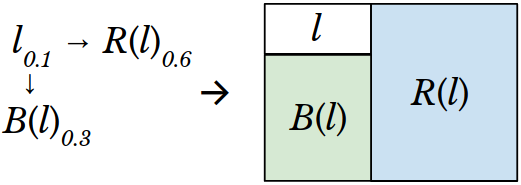
\includegraphics[width=.8\textwidth]{figures/treemap-algorithm/space-partition.png}
\caption{Space partitioning from $LT$.}
\label{fig:space-partition}
\end{figure}

GIT proceeds in two phases: initialization and update, as follows.\\

\noindent\textbf{Initialization:} To start with, we need to construct $LT$ from the first tree $T(t=0)$ in our sequence. For this, we can use basically any method ${\cal T}_{init}$ that constructs a (static) treemap for $T(0)$ from which we can next generate $LT$ with the properties (a) and (b) mentioned above. We have experimented with two such initialization methods. First, we constructed $LT$ from a squarified treemap (\emph{i.e.} ${\cal T}_{init}$ is the SQR algorithm), since SQR is well known to yield very good AR values. Alternatively, we propose a simple heuristic ${\cal T}_{init}^{direct}$ that directly builds $LT$ from the initial tree $T(0)$. Both initialization methods are compared next in Sec.~\ref{sec:results-3}.

To explain our heuristic ${\cal T}_{init}^{direct}$, consider a single-level tree $T = [(n_i,a_i)]  =  [ (A, 10), (B, 2), (C, 8), (D, 4), (E, 1), (F, 3) ]$, to be laid our, for simplicity, in a square drawing area $S$ of size 1; handling general trees is trivial by top-down recursion. We build $LT$ by sequentially adding each $n_i \in T$ to it (Fig.~\ref{fig:git_example}). After each addition, we rebuild ${\cal T}$ from the current $LT$ as explained above, so it covers the entire $S$. Thus, existing nodes are `squeezed' to make space for the new nodes. In our example, we first add node $A$, which will cover the entire $S$. To add $B$, we find the node $n \in LT$ having the worst aspect-ratio cell $c \in {\cal T}$. If $w_c \geq h_c$, we add $B$ directly right of $n$ (as in our example), else we add $B$ directly below $n$, and update ${\cal T}$ from the new $LT$ again. For the third node $C$, as the worst-aspect-ratio cell is $B$, and since $h_B > w_B$, we add $C$ below $B$ and update ${\cal T}$ from $LT$ again. Fig.~\ref{fig:git_example}(d-f) shows the addition of the remaining nodes of $T$.\\

\begin{figure}[htbp!]
\centering
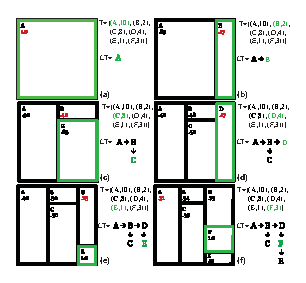
\includegraphics[width=.8\textwidth]{figures/treemap-algorithm/git_example.eps}
\caption{Building the initial layout tree $LT$ (green: inserted cells).}
\label{fig:git_example}
\end{figure}

For didactic purposes, nodes were added in alphabetical order, but in reality, we want nodes to be added in random order, hence when dealing with truly hierarchical data, one sub-tree is not completely laid out before its siblings, which could cause it to be `squeezed'.

\noindent\textbf{Update:} We now have an initial treemap ${\cal T}$ and its $LT$. We next edit $LT$ to handle weight changes, node additions, and node deletions as $T$ changes. \emph{Weight} changes do not change $LT$. \emph{Additions} are handled just as adding regular nodes when building the initial $LT$ using ${\cal T}_{init}^{direct}$. Additions tend to increase the cells' aspect ratios, so we do them after node removals and weight changes. \emph{Removals} are done by editing $LT$ as follows (see also Fig.~\ref{fig:git_removal}):

\begin{enumerate}
\item If a node $n\in LT$ has a $B(n)$ subtree, we replace $n$ by $B(n)$;
\item else if $n$ has a $R(n)$ subtree, we replace $n$ by $R(n)$;
\item else $n$ has no subtrees, so we just remove it from $LT$.
\end{enumerate}

After handling all changes in a new revision of $T$, we rebuild ${\cal T}$ from $LT$, as already explained. As we show next in Sec.~\ref{sec:results-3}, GIT scores a very good balance of spatial quality \emph{vs} stability.

\begin{figure}[htbp!]
\centering
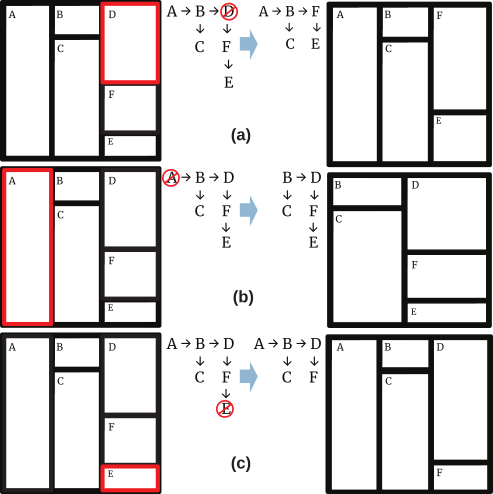
\includegraphics[width=.8\textwidth]{figures/treemap-algorithm/git_removal.eps}
\caption{Removal of nodes (red) from layout tree and its treemap.}
\label{fig:git_removal}
\end{figure}


\section{Evaluation}
\label{sec:evaluation}
%
To evaluate GIT, we considered the following aspects:

\subsection{Metrics}
\label{sec:eval_metrics}
%
To evaluate the quality of GIT, we proceed as follows. For spatial quality, we use the well-known Aspect Ratio metric ($AR$)~\cite{sqr}. For each cell $c$ in a treemap ${\cal T}$, $AR_c = min(w_c, h_c)/max(w_c, h_c)$. This metric is considered by virtually all rectangular treemap evaluations we are aware of.

For stability, we compute three metrics. The first two are the Shneiderman-Wattenberg's Layout Distance Change ($LDC$)~\cite{ordered} and Tak-Cockburn's Location Drift ($LD$)~\cite{hilbert_moore}, already introduced in
Sec.~\ref{sec:related_work}. The $LDC$ metric captures the instability of a cell between consecutive revisions. In contrast, the $LD$ metric captures the deviation of a cell's position over all timesteps.

We also propose a (new) third metric, which extends $LDC$ to also consider the change of the \emph{data}. We define the \emph{visual change} of a cell $c_i$ as the Euclidean distance traveled by the four corners of the rectangle $r_i$ between $t$ and $t+1$, normalized by the treemap diagonal $\sqrt{W^2+H^2}$, so $\delta v_i \in [0,1]$. Next, we define the \emph{data change} of $c_i$ as $\delta a_i = |a_i(t)-a_i(t+1)|$, where $a_i$ is the relative weight of node $c_i$. With these, we define the stability $Q_i$ of a cell $c_i$ in a treemap as

\begin{equation}
Q_i =  (1-\delta v_i) / (1 - \delta a_i).
\label{eqn:stab_ratio}
\end{equation}

We define the stability $Q$ of an entire treemap as the average of its cells' stabilities $Q_i$. In contrast to $LDC$, $Q$ measures how much a rectangle changes \emph{in relation to its data change}. Measuring only absolute changes of rectangles ($LDC$) does not, we believe, fully characterize stability. Indeed, a rectangle could (and should) change a lot if its underlying cell's weight changes a lot. However, this does not mean necessarily that the treemap algorithm is unstable.

\subsection{Techniques}
%
We tested GIT against 14 other treemapping algorithms: Approximate (APP), Hilbert (HIL), Stable treemaps (LM0, LM4), Moore (MOO), NMap-Alternate-Cuts (NAC), NMap-Equal-Weights (NEW), Pivot-by-Middle (PBM), Pivot-by-Size (PBZ), Pivot-by-Split-Size (PBS), Slice- and-Dice (SND), Spiral (SPI), Squarified (SQR), and Strip (STR). For NMap, we use as seed layout the one computed by SQR~\cite{nmap}. We did not consider non-rectangular treemap methods in the evaluation, since not all the metrics in Sec.~\ref{sec:metrics-3} directly generalize to non-rectangular cells.

\subsection{Datasets}
%
We extracted 28 dynamic hierarchies by mining the structure of software projects (folders, files, classes) from 28 corresponding public GitHub repositories, using a custom automated pipeline that scans all available revisions and extracts the code structure using Understand~\cite{understand}. As weights $w_i$, we use the number of lines of code of the respective items. Other software quality metrics delivered by Understand can be used instead, if desired. For more details on this process, we refer to~\cite{vmv}. The considered repositories have quite different sizes, number of revisions, hierarchy depths and shapes, number of developers, and code type (programming languages and application types). Statistics about the datasets are available in Table~\ref{tab:datasets-3}.

\begin{table}[htbp!]
\small
\centering
\scalebox{0.9}{
\begin{tabular}{|l|l|r|r|}
\hline
\textbf{Dataset} & \textbf{Revisions} & \textbf{Nodes (total)} & \textbf{Average depth} \\
\hline
animate.css & 50 & 3454 & 2.87\\
AudioKit & 22 & 11178 & 6.95\\
bdb & 62 & 2658  & 3.83\\
beets & 106   & 9844 & 3.75\\
brackets &  88  & 120292 & 12.85\\
caffe & 44 & 12969   & 4.93\\
calcuta & 50 & 2882 & 10.76\\
cpython   & 321 & 584821 & 6.50\\
earthdata-search   &  46& 18539 & 6.82\\
emcee & 64 & 1746  & 3.62\\
exo & 97 &  36436  & 11.88\\
fsharp   & 69 & 22906 & 7.89\\
gimp   & 72 &  170418 & 5.19\\
hospitalrun-frontend   & 38 &  16759 & 5.71\\
Hystrix & 61 & 15530  & 13.29\\
iina & 74 &  6849  & 4\\
jenkins & 137  & 277185 & 11.94 \\
Leaflet &  84  & 13381 & 4.86 \\
OptiKey   & 36 & 9782 & 6.72\\
osquery  & 37 & 14111 & 5.75 \\
PhysicsJS   & 20 & 2022 & 4.6\\
pybuilder   & 53 & 5457 & 7\\
scikitlearn   & 88 & 48468 & 5.75\\
shellcheck   & 53 & 746 & 2.39\\
soundnode-app   & 35 & 3196 & 6.88\\
spacemacs   & 51 & 10201 & 4.96\\
standard   & 29 & 203 & 2\\
uws & 122 & 4093 & 2.76\\
\hline
\hline
\textbf{Totals:} & 2132 & 1458036 & 5.77\\
\hline
\end{tabular}
}
\caption{Software evolution tree datasets used in the evaluation.}
\label{tab:datasets-3}
\end{table}


\section{Results}
\label{sec:results-3}
%
We evaluate GIT on the aforementioned datasets, algorithms, and metrics collection from several perspectives, by answering a series of questions. Below, average stability $S$ refers to the average of the $LDC$ and $Q$ metrics introduced in Sec.~\ref{sec:metrics-3}. All results that we were not able to fit in the paper can be found at our online repository\cite{benchmark}.

\subsection{How does GIT's initialization affect its quality?}
%
As outlined in Sec.~\ref{sec:git}, we can initialize GIT with various treemap layouts, such as squarified (SQR) or using the direct initialization illustrated in Fig.~\ref{fig:git_example}. Intuitively, one would think that SQR initialization is to be preferred, since SQR is well known for its high $AR$ values. To test this, we ran GIT using both initializations for all datasets. After initialization, the same regular GIT update mechanism is used in both cases. Figure~\ref{fig:git_vs_sqr} shows the per-dataset average stability and $AR$ values. Interestingly, we see that the higher-$AR$ SQR initialization actually yields slightly worse $AR$ values for the entire sequence. For stability, the two initializations behave basically identically. We can explain this result by the fact that the GIT direct initialization follows the same heuristics as the update steps, while SQR forces GIT to start with a layout which needs more substantial updates next as the tree data changes. At a higher level, this experiment suggests that GIT performs very well using direct initialization. As such, we use this initialization in all subsequent experiments.

\begin{figure}[htbp!]
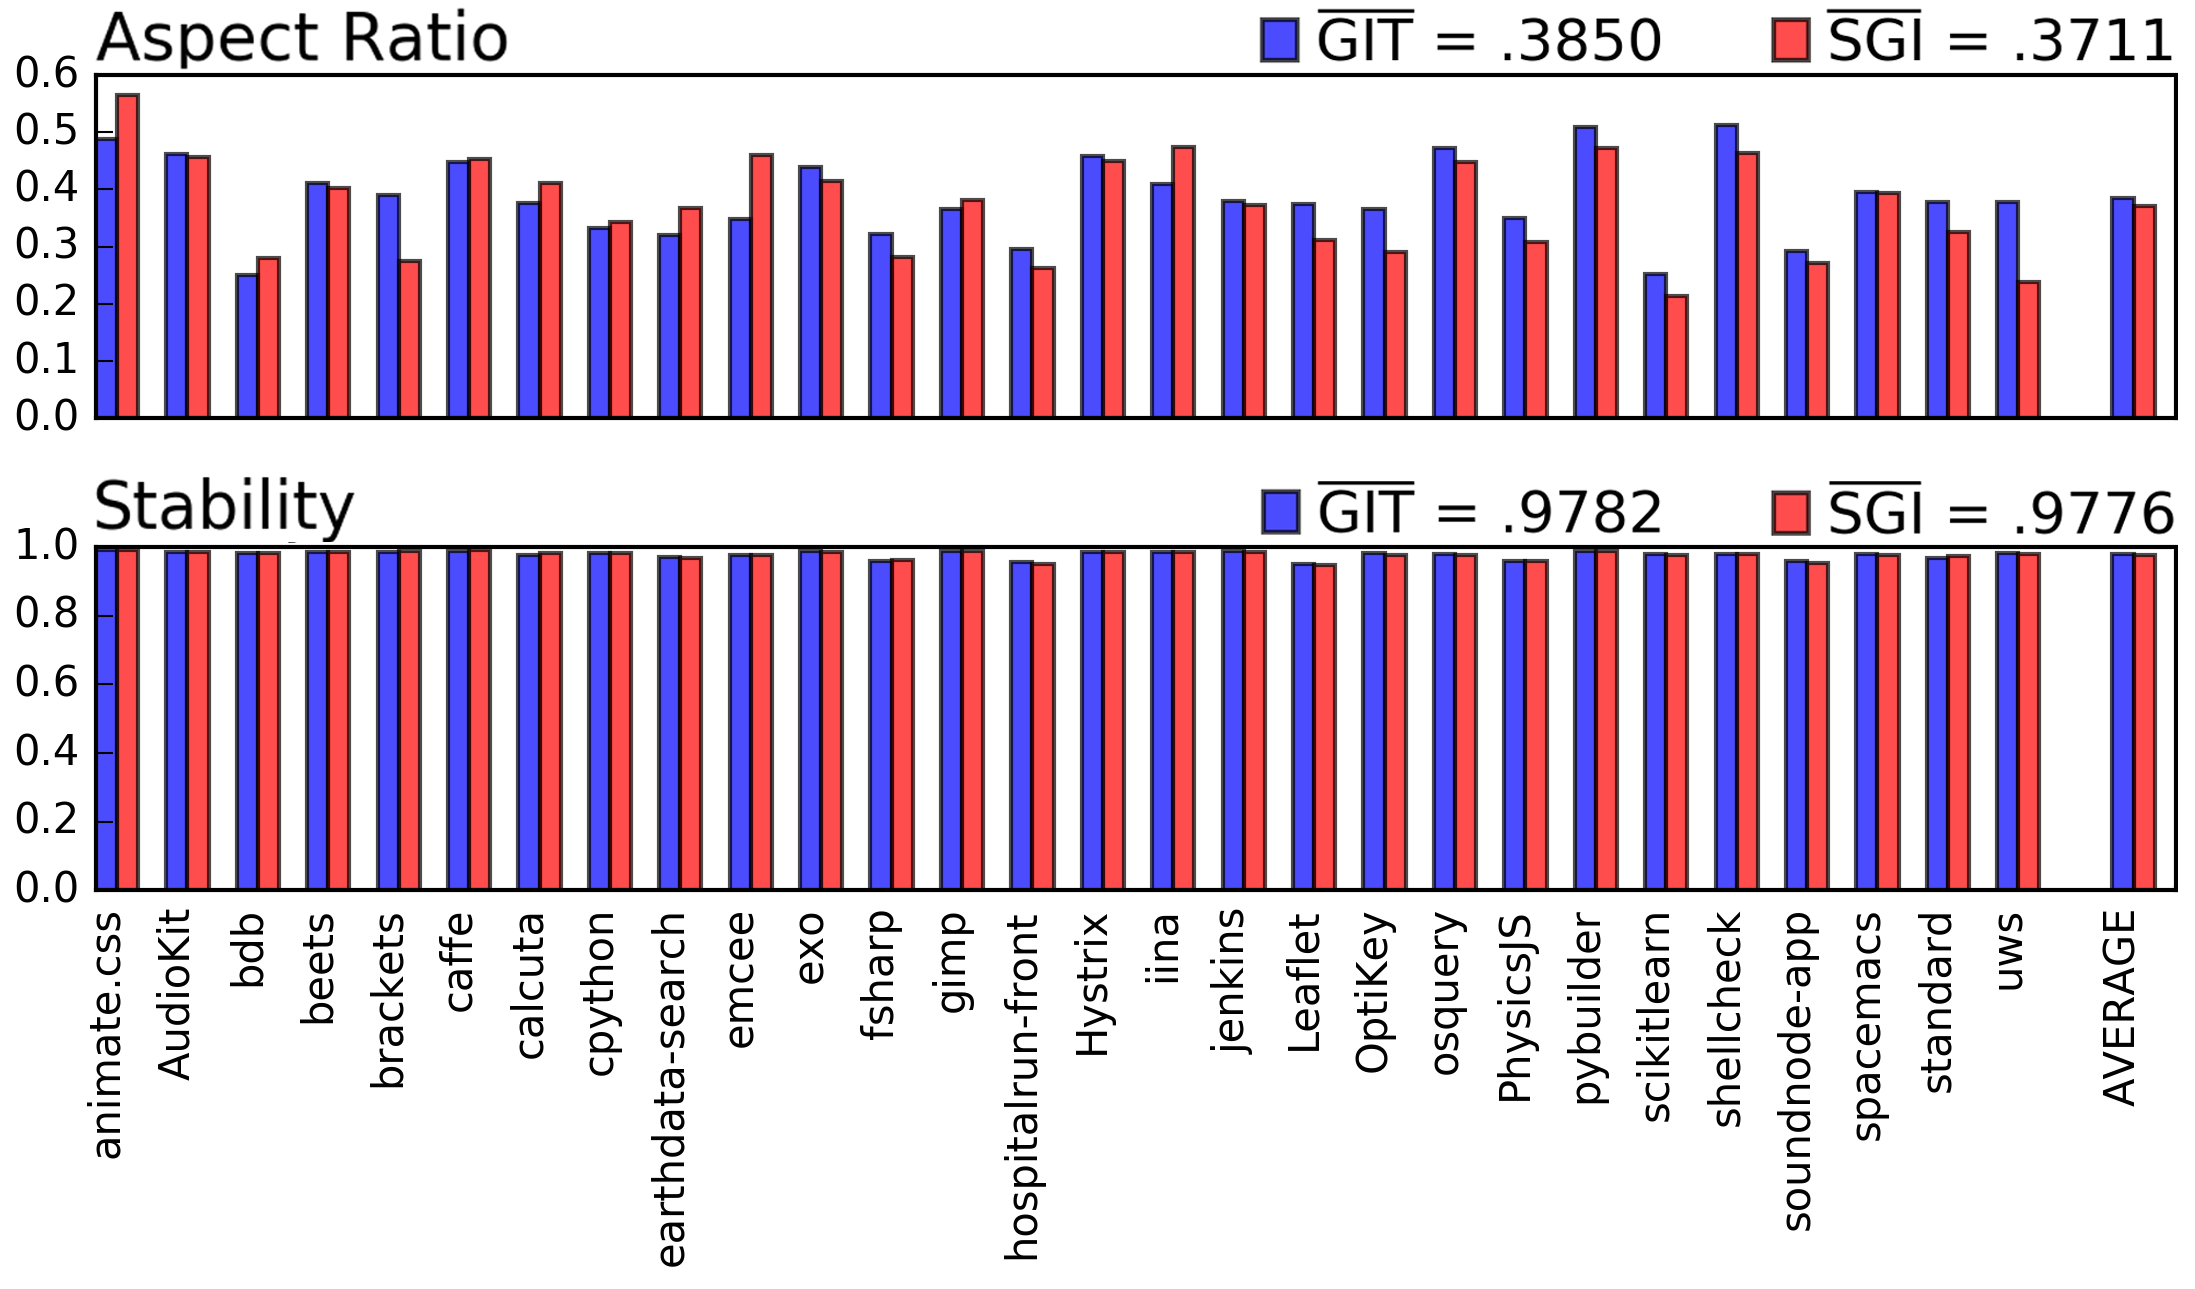
\includegraphics[width=.48\textwidth]{figures/treemap-algorithm/git-vs-sqrgit-both.png}
\caption{GIT performance using ${\cal T}_{init}^{direct}$ (GIT) \emph{vs} squarified initialization (SGI). }
\label{fig:git_vs_sqr}
\end{figure}

\subsection{How do visual quality and stability vary over time?}
%
As we have already noted, spatial quality and stability are roughly inversely correlated desiderates -- a treemap that scores well for one of these metrics tends to score less well for the other one. Hence, comparing how these metrics change in time is interesting. To answer this, we display, for one dataset and all tested algorithms, two charts showing the median (black), 25-75\% range (green), and 5-95\% range (gray) of the $AR$ and $S$ metrics (Fig.~\ref{fig:boxplots}). We see that APP and SQR have the best $AR$ values, and SND the worst $AR$ values. The other algorithms, including GIT, score in-between. In contrast, GIT, LM0, and SND score the best for stability, while all other algorithms exhibit a non-negligible number of unstable time moments. This suggests that GIT strikes a good compromise between stability and aspect ratio.

\begin{figure*}[htbp!]
\centering
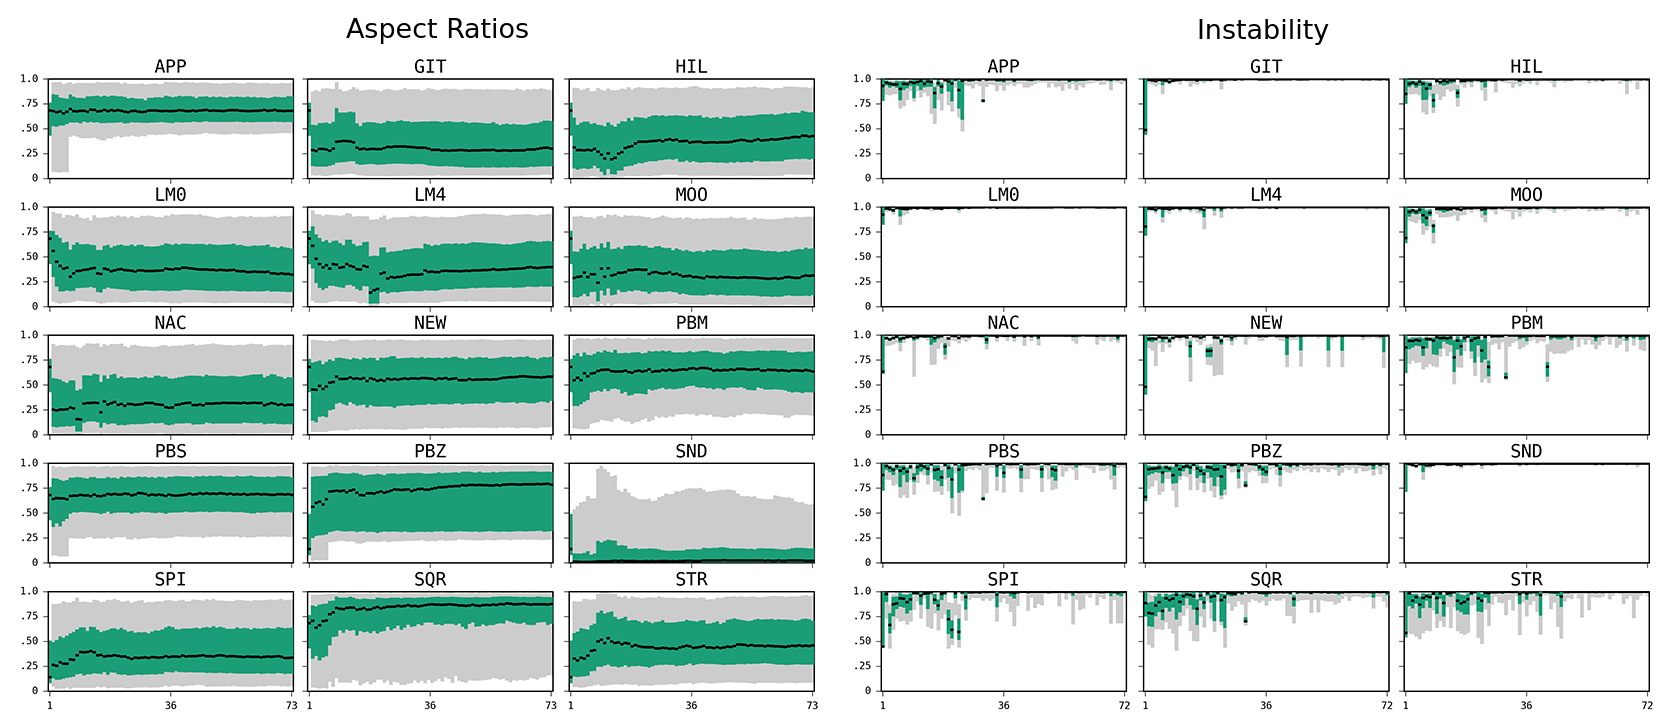
\includegraphics[width=\textwidth]{figures/treemap-algorithm/boxplots-gimp.png}
%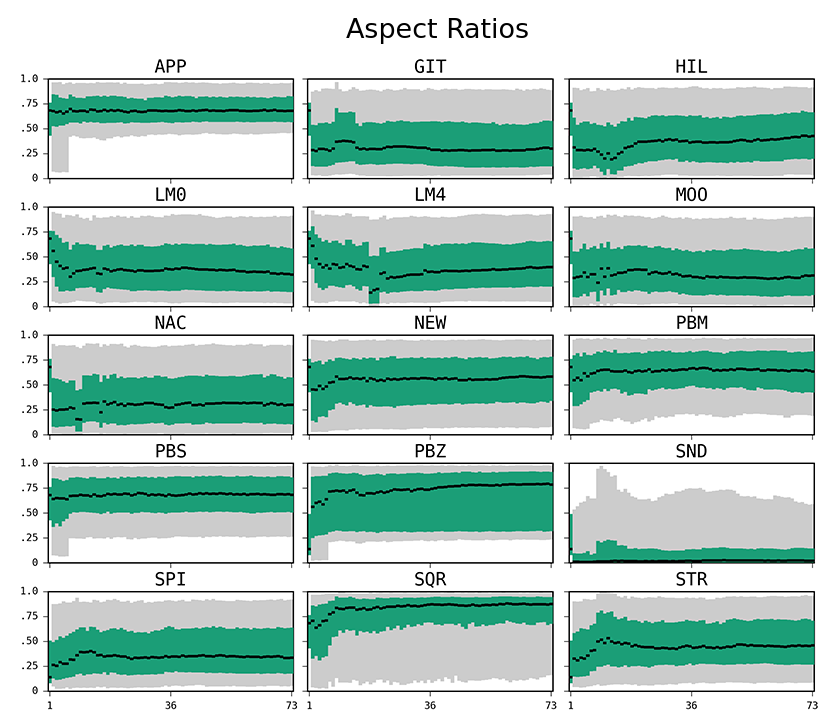
\includegraphics[width=0.69\linewidth]{figures/boxplots-gimp-ar.png}
%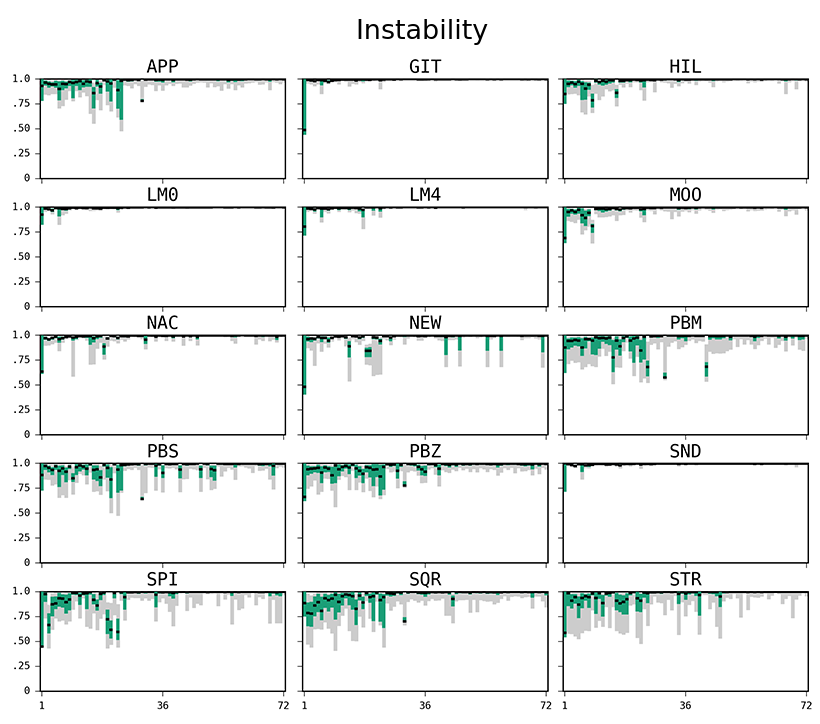
\includegraphics[width=0.69\linewidth]{figures/boxplots-gimp-st.png}
\caption{Distribution of aspect ratio ($AR, left$) and average stability ($S$, right) values over time for the GIMP dataset.}
\label{fig:boxplots}
\end{figure*}

While Fig.~\ref{fig:boxplots}(right) shows how the per-timestep stability changes over time, it does not show us which actual instability patterns each method is prone to deliver. Knowing this is useful, as we can better understand what to expect in terms of (undesired) cell moves from a certain algorithm, including GIT. To show this, we plot the trails connecting all centers $k_i(t)$ of all rectangles $r_i(t)$ for consecutive $t$ values over a given tree sequence (Fig.~\ref{fig:centroids}). We set the opacity of each line segment $(r_i(t), r_i(t+1))$ to the Euclidean distance $\| k_i(t) - k_i(t+1)\|$ normalized by the square root of the number of time steps. Hence, dark long lines show big moves (instability) while small moves (close to stability) are hardly visible. The image confirms the high stability of GIT --  in contrast to most other methods, except SND, GIT creates smaller cell moves (shorter dark lines), and most of these are close to horizontal or vertical. Interestingly, we see that other methods create quite different move patterns: SQR, PBS, PBZ, and PBM have mostly (large) diagonal moves. SPI shows a coil-like movement and in STR we see no vertical travel. Overall, we see that GIT is more stable not only because it yields smaller moves, but also because it constrains these to fewer motion directions, thus causes less complex dynamics (that the user must follow) in the resulting visualization. This can be also checked by watching the actual videos showing the algorithms in action~\cite{benchmark}.

\begin{figure*}[htbp!]
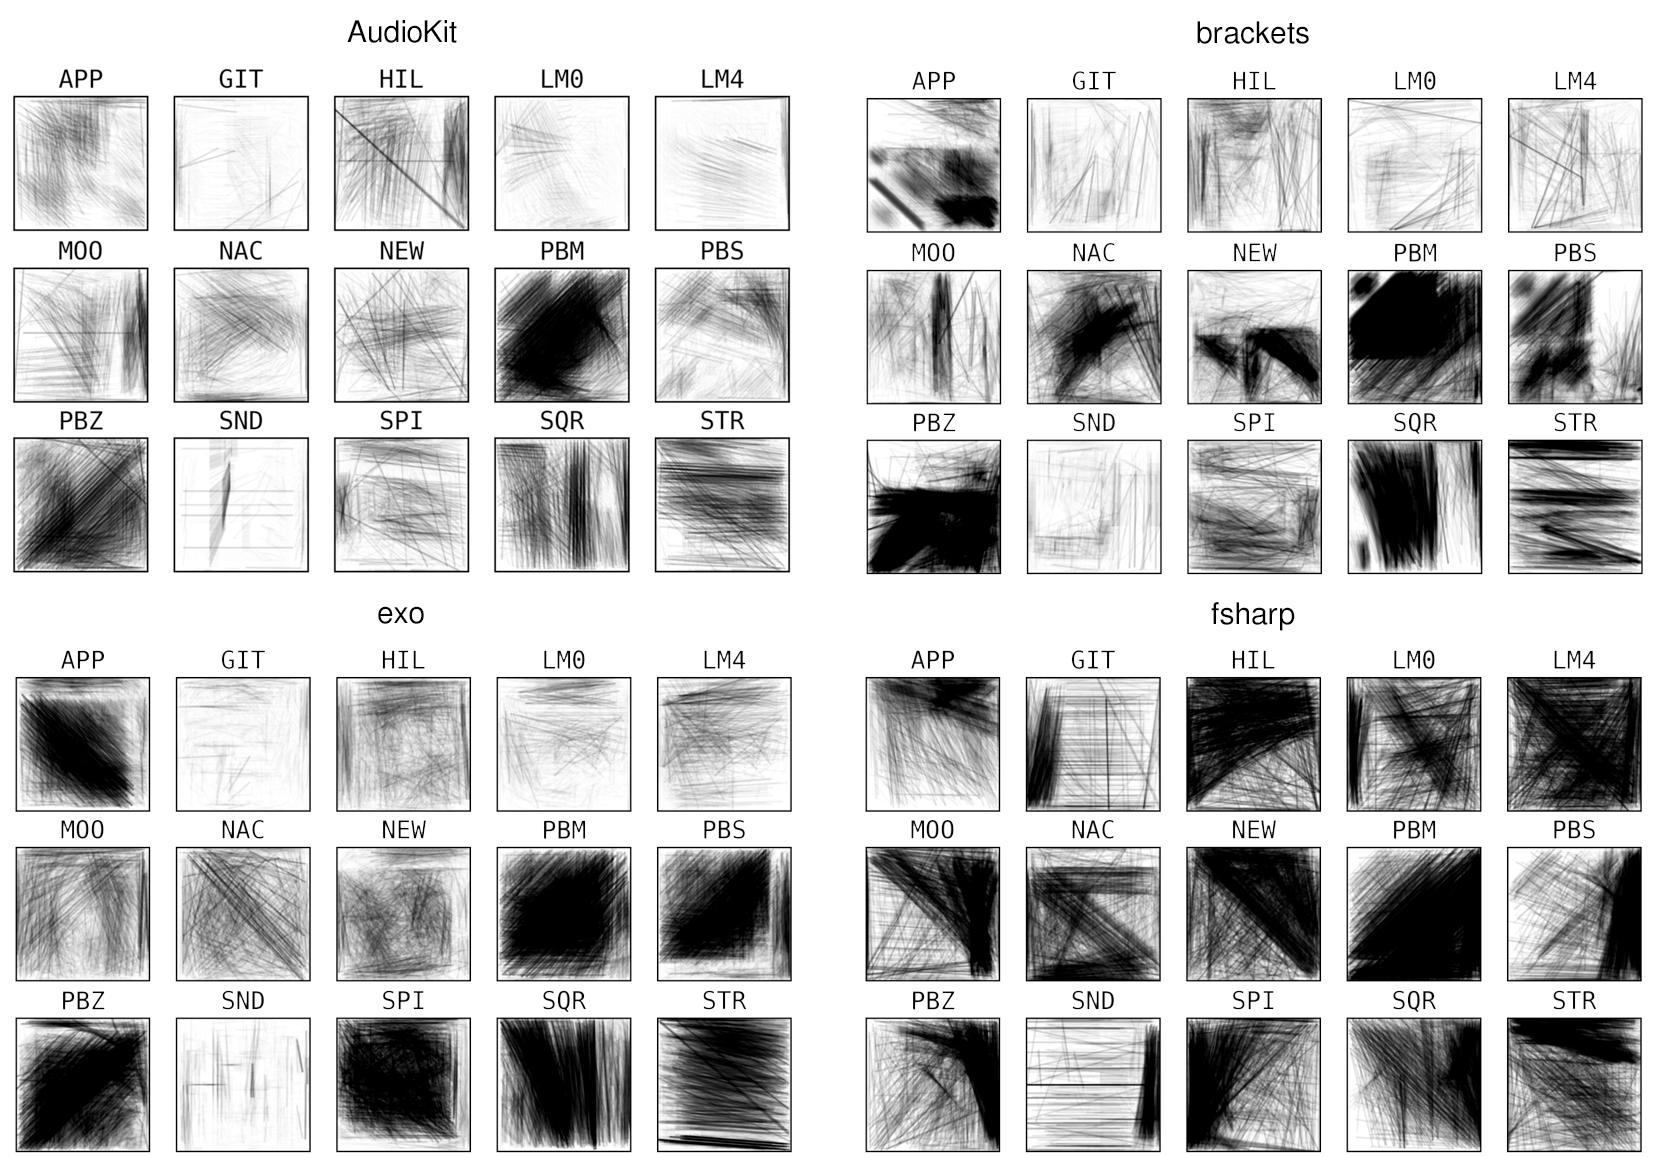
\includegraphics[width=\textwidth]{figures/treemap-algorithm/centroid-4.png}
\caption{Instability (cell center motion) patterns, all methods, \emph{AudioKit}, \emph{brackets}, \emph{exo} and \emph{fsharp} datasets.}
\label{fig:centroids}
\end{figure*}

\subsection{How do all quality metrics vary over all datasets?}
%
The experiments so far do not show the individual stability metrics (including $LD$, which can be only computed for an entire sequence), nor, for space reasons, the metrics over all 28 tested tree sequences. To get more insight in how GIT performs in these respects, we show the per-dataset average values (for $AR$ and the three stability metrics) for all tested methods, all datasets (Fig.~\ref{fig:tables}). Cells are colored using a purple (low values) to yellow (high values) colormap. We observe the following: For $AR$, APP scores consistently better for most datasets than all other tested methods. SQR reaches the highest $AR$ values, but only for a very few datasets. SND, as expected, scores overall the poorest. The remaining methods can be divided roughly into two groups, with NEW, PBM, PBS, STR, and PBZ scoring overall higher than GIT, HIL, LM0, LM4, MOO, and NAC. Concerning stability, SND scores consistently the best for all three considered metrics, and GIT, LM0, and LM4 come in the second place. This strengthens our earlier observation that GIT strikes a good balance between stability and spatial quality.

\begin{figure}[htbp!]
%\includegraphics[width=.5\textwidth]{figures/tables.png}
\includegraphics[width=1.0\linewidth]{figures/treemap-algorithm/tables.png}
\caption{Average metric values for all techniques and all datasets.}
\label{fig:tables}
\end{figure}

\subsection{How to summarize GIT's quality?}
%
As noted, GIT seems to strike a good balance between spatial quality and stability. We summarize both these metrics for GIT and all other algorithms using a star plot (Fig.~\ref{fig:star-3}). The figure shows a scatterplot with $x$ mapping average stability $S$ and $y$ aspect ratio $AR$, respectively. Categorically colored points, one color per method, indicate the tested methods, attributed by their $S$ and $AR$ values over all datasets, all time steps. From each point (method), we draw lines connecting it with the $S$ and $AR$ values obtained for all the 28 tested datasets. A good algorithm has thus its `star' center placed top-right and relatively short star arms, indicating consistent quality over the entire dataset collection. We see several patterns, as follows.

At a high level, stability is roughly inversely correlated with spatial quality -- methods that score very well on one tend to score worse on the other. We see three groups of methods: APP, PBS, SQR, PBM, STR, PBZ and NEW score well on spatial quality, but poorly (except NEW) on stability. SND is the opposite outlier, scoring best on stability but clearly poorest on spatial quality. A middle group of methods (GIT, LM0, LM4, MOO, NAC, SPI, and HIL) trades well stability \emph{vs} spatial quality. Within these, GIT scores the best stability, and LM0 the best spatial quality. As such, GIT and LM0 can be considered complementary methods with respect to the stability \emph{vs} spatial quality trade-off. However, LM0 has a considerably more complex and slower implementation than GIT -- for details, we refer to~\cite{sondag17}. Separately, we see that GIT's star size (convex hull containing the lines emerging from the GIT point) is one of the smallest of all tested methods. Hence, GIT offers one of the most consistent behaviors over the entire dataset collection from all tested algorithms.

\begin{figure}[htbp!]
  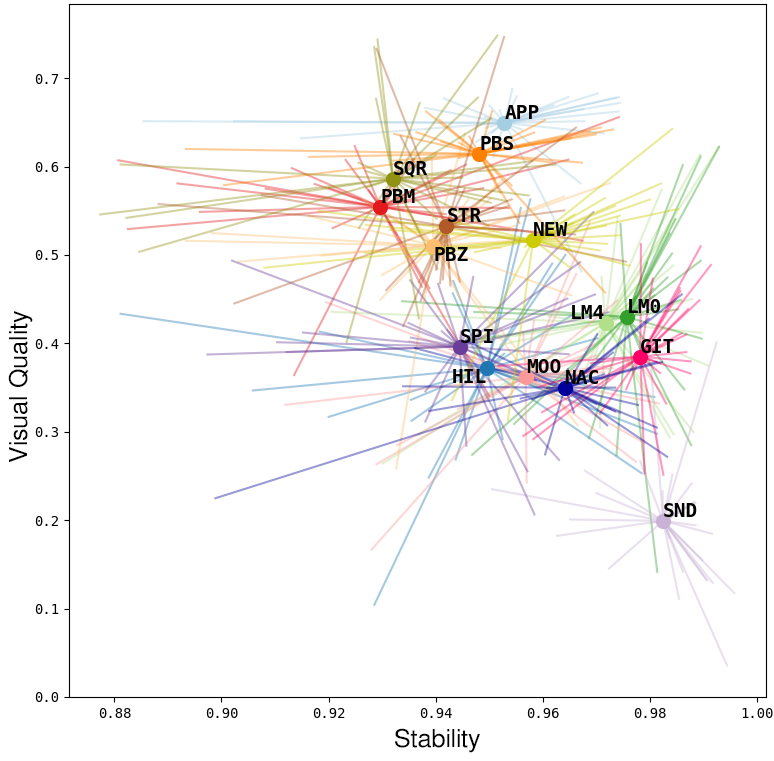
\includegraphics[width=1.0\linewidth]{figures/treemap-algorithm/star.png}
\caption{Star plot summarizing both visual quality and stability, all algorithms, all datasets.}
\label{fig:star-3}
\end{figure}

\section{Conclusion}
\label{sec:conclusion-3}
We have presented a new method for computing treemap layouts for time-dependent hierarchies. As discussed earlier, there are only a few methods in the literature that consider quality aspects pertaining to \emph{both} spatial quality and stability of such treemaps. Our contribution, in brief, is proposing a new method that takes both these quality aspects into account; and evaluating our method comprehensively on a broad dataset of 28 time-dependent hierarchies extracted from real-world dynamic dataset (software repositories), against 14 well-known treemapping methods, and using 4 quality metrics. Our results show that our new method strikes a good balance between spatial quality and stability as compared to state-of-the-art methods. Additionally, our method is simple to implement, fast, generic (with respect to the considered dynamic hierarchies), and has no hidden free parameters. More importantly, our method is an addition of a very small set of so-called \emph{stateful} methods that consider the evolution of a dynamic tree sequence when computing suitable treemaps thereof. Most existing treemapping methods are not designed to consider tree state, which arguably makes them suboptimal for handling inherently stateful datasets like dynamic trees.

Several future work directions are possible, as follows. Firstly, it is interesting to extend our evaluation to dynamic hierarchies from other domains than software evolution. This may show how much our proposal can effectively handle such more diverse datasets. Secondly, we argue that more refined quality metrics are needed (in general, for our new method but also any other treemapping methods) to capture the quality of such methods, as perceived by end users and in sync with their tasks. Finally, understanding the trade-off between the (algorithmic) reasons behind spatial quality and stability, \emph{i.e.} what to do to optimally satisfy both these requirements, is an open problem, to which we believe to have contributed to with our current work.

\begingroup
\let\clearpage\relax
\let\cleardoublepage\relax
\let\cleardoublepage\relax

\manualmark
\markboth{\spacedlowsmallcaps{Projection Evaluation}}{\spacedlowsmallcaps{Projection Evaluation}} 
\phantomsection 

\pdfbookmark[0]{Projection Evaluation}{projection-evaluation}
\chapter*{Projection Evaluation}

Lorem ipsum dolor sit amet, consectetur adipiscing elit, sed do eiusmod tempor incididunt ut labore et dolore magna aliqua. Ut enim ad minim veniam, quis nostrud exercitation ullamco laboris nisi ut aliquip ex ea commodo consequat. Duis aute irure dolor in reprehenderit in voluptate velit esse cillum dolore eu fugiat nulla pariatur. Excepteur sint occaecat cupidatat non proident, sunt in culpa qui officia deserunt mollit anim id est laborum.

\newpage

\endgroup
\begingroup
\let\clearpage\relax
\let\cleardoublepage\relax
\let\cleardoublepage\relax

\manualmark
\markboth{\spacedlowsmallcaps{Projection Algorithm}}{\spacedlowsmallcaps{Projection Algorithm}} 
\phantomsection 

\pdfbookmark[0]{Projection Algorithm}{projection-algorithm}
\chapter*{Projection Algorithm}

Lorem ipsum dolor sit amet, consectetur adipiscing elit, sed do eiusmod tempor incididunt ut labore et dolore magna aliqua. Ut enim ad minim veniam, quis nostrud exercitation ullamco laboris nisi ut aliquip ex ea commodo consequat. Duis aute irure dolor in reprehenderit in voluptate velit esse cillum dolore eu fugiat nulla pariatur. Excepteur sint occaecat cupidatat non proident, sunt in culpa qui officia deserunt mollit anim id est laborum.

\newpage

\endgroup
%\include{chapters/6-fourth-project}
%\include{chapters/7-conclusion}

% Backmatter
\backmatter
\cleardoublepage\manualmark
\markboth{\spacedlowsmallcaps{\bibname}}{\spacedlowsmallcaps{\bibname}} 
\phantomsection 

\refstepcounter{dummy}
\addtocontents{toc}{\protect\vspace{\beforebibskip}}
\addcontentsline{toc}{chapter}{\tocEntry{\bibname}}

\bibliographystyle{plainabbrvnat}
\bibliography{bibliography-eurovis-treemaps.bib}

\cleardoublepage\manualmark
\markboth{\spacedlowsmallcaps{Acknowledgments}}{\spacedlowsmallcaps{Acknowledgments}} % work-around to have small caps also

\begingroup
\let\clearpage\relax
\let\cleardoublepage\relax
\let\cleardoublepage\relax

\chapter*{Acknowledgments}
\addcontentsline{toc}{chapter}{\texorpdfstring{\spacedlowsmallcaps{Acknowledgments}}{Acknowledgments}}

I would like to thank my advisors Prof. Alexandru Telea and Prof. Jo\~{a}o Comba for all the support and guidance they so skillfully and kindly provided to me during my PhD. I couldn't possibly imagine better companions for this journey.

I would like to thank my family for their love, their patience, their inspiration, and for always providing me all I've ever needed to succeed.

I would also like to thank all my friends both in Brazil and in the Netherlands. Krislen, Lianne, Alister, Samuel, Stefan, and Agathe, thank you for lifting me up whenever I was down.


\bigbreak

This thesis was financed in part by CAPES (Finance Code 001, Scholarship Code 88882.345509/2019-01), CNPq (Process 304336/2019-0), and by the University of Groningen. 
My sincere thanks to these organizations for their support.

\endgroup




\cleardoublepage\pagestyle{empty}

\null
\vfill

\pdfbookmark[0]{Colophon}{colophon}
\section*{Colophon}
This document was typeset using the typographical look-and-feel \texttt{classicthesis} developed by Andr\'e Miede. 
The style was inspired by Robert Bringhurst's seminal book on typography ``\emph{The Elements of Typographic Style}''. 
\texttt{classicthesis} is available for both \LaTeX\ and \mLyX: 
\begin{center}
\url{http://code.google.com/p/classicthesis/}
\end{center}
\noindent\finalVersionString

\end{document}


% FIXES:
% Section number not showing